% tikz pulls in xcolor itself, so the table option has to be registered before any package loads it.
\PassOptionsToPackage{table}{xcolor}
\documentclass[10pt]{article}

\usepackage{tmlr}
% On acceptance: \usepackage[accepted]{tmlr}. For a preprint: \usepackage[preprint]{tmlr}.
\usepackage{amsmath}
\usepackage{amssymb}
\usepackage{amsthm}
\usepackage{bm}
\usepackage{booktabs}
\usepackage{graphicx}
\usepackage{xcolor}
\usepackage{tikz}
\usetikzlibrary{arrows.meta,positioning,calc,fit,backgrounds,shapes.geometric,decorations.pathreplacing}
\definecolor{amber}{RGB}{240,180,40}

% Table shading. Light tints behind black text, rather than coloured numerals: the text stays fully
% legible, the ramp survives greyscale printing as a grey gradient, and a single-hue lightness ramp
% is readable under every common form of colour vision deficiency. Hues are the Okabe--Ito
% bluish-green and vermillion, which stay distinguishable to deuteranopes and protanopes.
\definecolor{hgood}{RGB}{0,145,105}
\definecolor{hbad}{RGB}{205,85,15}
\definecolor{hflat}{RGB}{70,90,125}
% #1 is the tint strength in percent; keep it under ~45 so the cell never fights the numeral.
\newcommand{\cgood}[2]{\cellcolor{hgood!#1}#2}
\newcommand{\cbad}[2]{\cellcolor{hbad!#1}#2}
\newcommand{\cflat}[1]{\cellcolor{hflat!13}#1}
\usepackage{url}
\usepackage[colorlinks=true,linkcolor=blue,citecolor=blue,urlcolor=blue]{hyperref}

\newtheorem{proposition}{Proposition}
\newtheorem{corollary}{Corollary}

\DeclareMathOperator{\KL}{KL}
\DeclareMathOperator{\TV}{TV}
\newcommand{\R}{\mathbb{R}}
\newcommand{\E}{\mathbb{E}}
\newcommand{\dd}{d}
\newcommand{\kk}{k}
% Marks a headline result. \bm rather than \mathbf so that operators such as \times bold too.
\newcommand{\best}[1]{\bm{#1}}

\title{The Dimensionality Barrier in Continuous Speculative Sampling}

% Under review the tmlr package prints "Anonymous authors" and ignores this block; it is
% typeset only under the [accepted] or [preprint] options.
\author{\name Author One \email one@example.edu \\
      \addr Department\\
      Institution}

\def\month{MM}
\def\year{YYYY}
\def\openreview{\url{https://openreview.net/forum?id=XXXX}}

\begin{document}

\maketitle

\begin{abstract}
Speculative sampling accelerates autoregressive generation without changing the output distribution,
which makes it the natural remedy for continuous-token image models such as MAR, where a sequential
per-token diffusion head consumes almost all of the wall time. We show that exact acceptance instead
deteriorates rapidly with the token dimension. In a controlled dimension-indexed sweep, acceptance
falls $\best{181\times}$ as the token widens from $\dd{=}4$ to $\dd{=}128$ while the per-coordinate
draft--target disagreement stays flat, and a training-free Gaussian reference reproduces the same
curve out to $\dd{=}4096$. We then ask whether the natural repair works: verify only a
low-dimensional projection of each token, as transform coding keeps a low-frequency band and discards
the rest. It cannot remove the obstruction. Splitting a token into a verified statistic and its
complement leaves the total draft--target divergence exactly unchanged, by the chain rule for KL and
with no Gaussian assumption; projection converts divergence that the test would have seen into
divergence that escapes it. For shared-covariance Gaussians this becomes a closed-form
acceptance--fidelity frontier, and a subspace rule can only choose a point on that frontier rather
than move it. Across five substantially different rules, including the low-frequency DCT band and an
adversarial anti-control that verifies the least important directions, measured costs span $48$ nats
yet every rule lies within $\best{4.0\%}$ of a single curve. Two further measurements support the
same reading: the KL16 decoder MAR uses shows no compact perceptual band among the top $64$ of
$4096$ latent directions, and distilling the draft towards the target, which changes the divergence
itself rather than where it is paid, moves the frontier and raises lossless acceptance by
$\best{5.72\times}$ at $\dd{=}128$ at zero fidelity cost. The practical consequence is a feasibility
rule: holding acceptance at $0.5$ demands per-coordinate agreement within $0.34\sigma$ at
$\dd{=}16$ but within $0.021\sigma$ at $\dd{=}4096$, so for continuous speculative verification
reducing draft--target divergence matters more than designing a better projection.
\end{abstract}

\section{Introduction}
\label{sec:intro}

Autoregressive image generation now rivals diffusion, and it has inherited diffusion's latency. A
masked autoregressive model such as MAR \citep{li2024autoregressive} synthesises a $256 \times 256$
image by predicting a grid of \emph{continuous} latent tokens, one KL16 autoencoder token per patch,
and drawing each from a small per-token diffusion head. Instrumenting MAR-B at its published sampling
settings, we measure $98.3\%$ of wall-clock time inside that head. It dominates not by arithmetic
volume, since the transformer performs $4.5\times$ more token evaluations, but because its hundred
denoising steps are \emph{sequential} and run at a batch of one or two tokens. The passes cannot be
overlapped, and generation costs of order a minute per image. Latency, not throughput, is the
bottleneck.

Speculative sampling \citep{leviathan2023fast,chen2023accelerating} is the standard cure for this
disease, and it is a remarkable one because it costs nothing in quality. A cheap draft model proposes
a token $x \sim q$, an expensive target model scores it, and the proposal is accepted with
probability $\min\{1, p(x)/q(x)\}$; on rejection one draws from the residual $r \propto (p-q)_+$. The
scheme emits exactly $p$, so the speedup is free of any fidelity cost, and the expected acceptance
rate is $1 - \TV(p, q)$.

% System overview. Kept in its own file because it is long and iterated on independently of the
% prose. Coordinates are absolute and chosen so the picture is ~14cm wide, i.e. it reaches \textwidth
% at roughly unit scale; resizing much below 1 makes the annotation text illegible in print.
\begin{figure}[t]
\centering
\resizebox{\textwidth}{!}{%
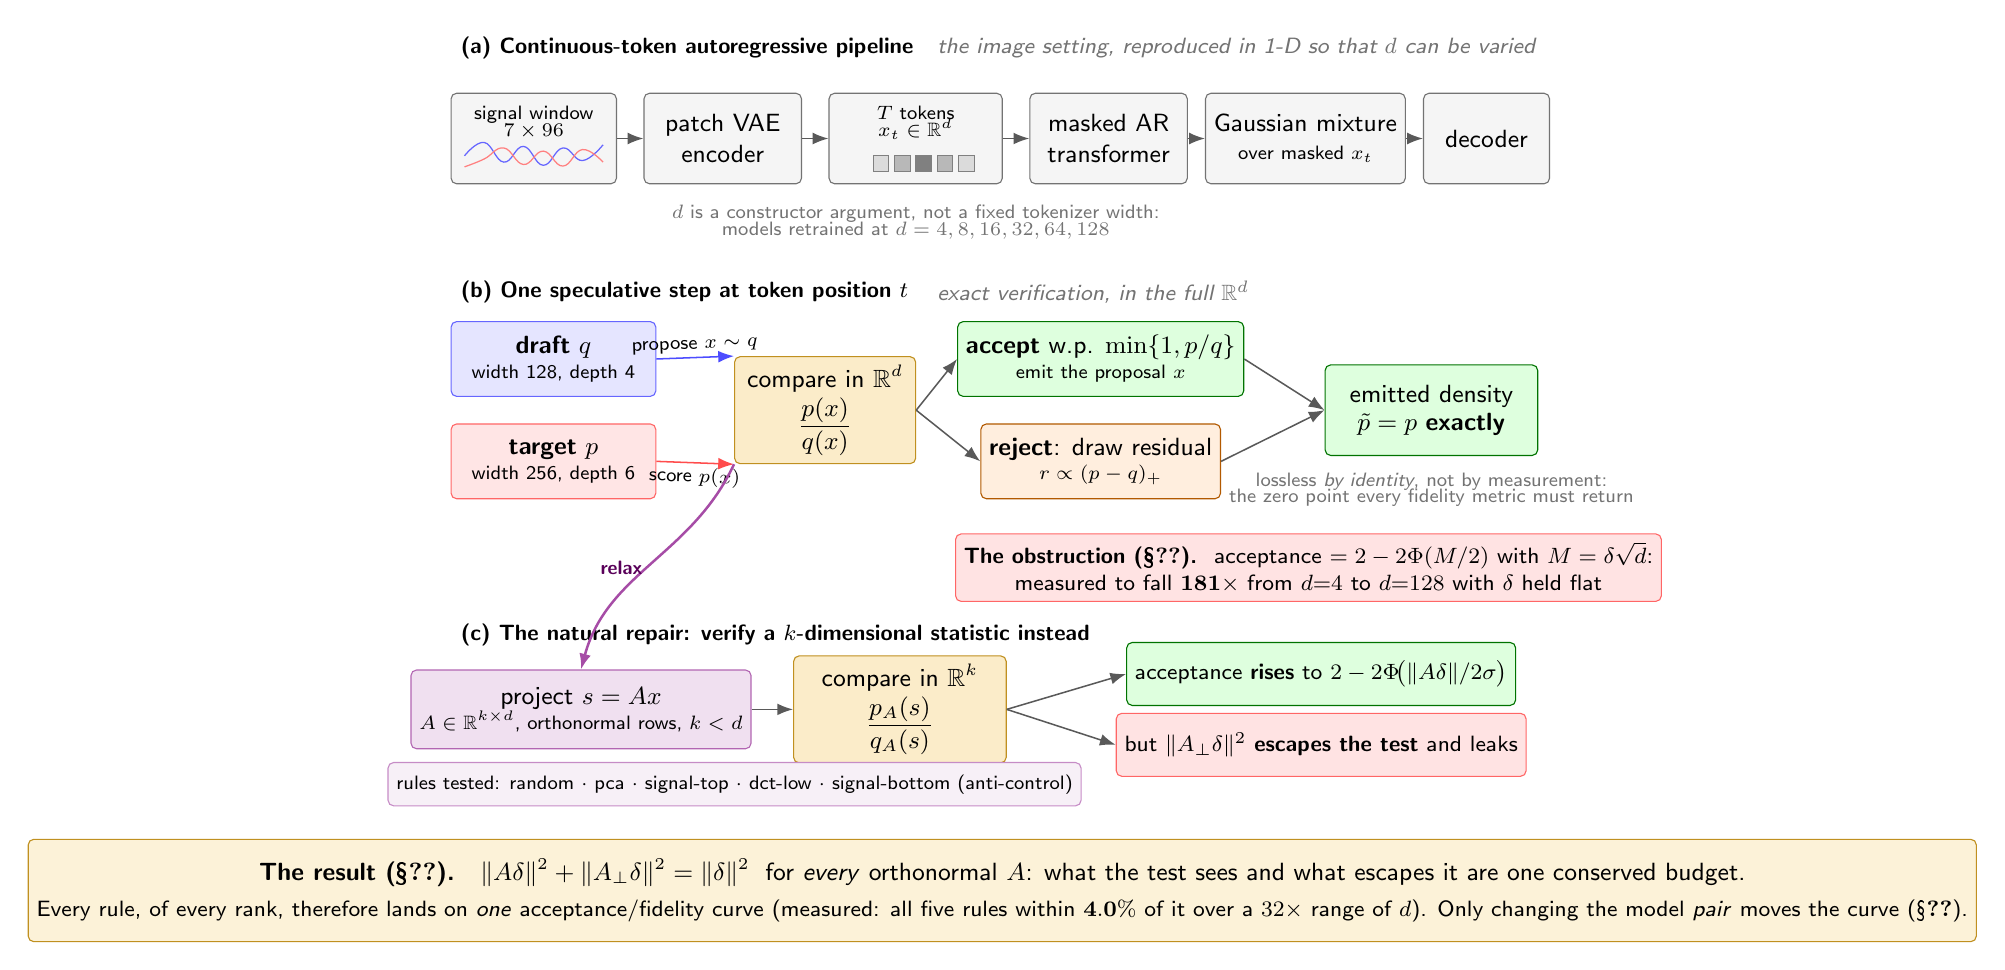
\begin{tikzpicture}[
  font=\sffamily\small,
  box/.style   = {draw=black!55, rounded corners=2pt, align=center, inner sep=3pt, fill=white},
  stage/.style = {box, fill=black!4, minimum height=1.15cm},
  draft/.style = {box, fill=blue!10,   draw=blue!60,        minimum height=0.95cm},
  targ/.style  = {box, fill=red!10,    draw=red!60,         minimum height=0.95cm},
  test/.style  = {box, fill=amber!25,  draw=amber!80!black},
  good/.style  = {box, fill=green!13,  draw=green!45!black},
  warn/.style  = {box, fill=orange!13, draw=orange!70!black},
  bad/.style   = {box, fill=red!11,    draw=red!60},
  proj/.style  = {box, fill=violet!12, draw=violet!60},
  fl/.style    = {-{Latex[length=2.0mm]}, draw=black!65, line width=0.55pt},
  hd/.style    = {font=\sffamily\bfseries\footnotesize, anchor=west},
  sub/.style   = {font=\sffamily\footnotesize\itshape, text=black!55, anchor=west},
  note/.style  = {font=\sffamily\scriptsize, text=black!55, align=center},
  lbl/.style   = {font=\sffamily\scriptsize, inner sep=1.5pt},
]

%======================= (a) the generative pipeline =======================
\node[hd]  at (0,2.15) {(a) Continuous-token autoregressive pipeline};
\node[sub] at (6.05,2.15) {the image setting, reproduced in 1-D so that $\dd$ can be varied};

\node[stage, minimum width=2.10cm] (sig) at (1.05,1.0)  {};
\node[font=\sffamily\scriptsize, anchor=north, align=center] at ($(sig.north)+(0,-0.05)$)
     {signal window\\[-2pt]$7 \times 96$};
\begin{scope}[shift={(sig.center)}]
  \draw[blue!60, line width=0.45pt] plot[smooth,tension=0.75]
    coordinates {(-0.88,-0.22) (-0.63,-0.05) (-0.38,-0.30) (-0.13,-0.10)
                 (0.12,-0.34) (0.37,-0.12) (0.62,-0.28) (0.88,-0.08)};
  \draw[red!50, line width=0.45pt] plot[smooth,tension=0.75]
    coordinates {(-0.88,-0.36) (-0.63,-0.26) (-0.38,-0.12) (-0.13,-0.33)
                 (0.12,-0.16) (0.37,-0.35) (0.62,-0.14) (0.88,-0.30)};
\end{scope}

\node[stage, minimum width=2.00cm] (enc) at (3.45,1.0) {patch VAE\\encoder};

\node[stage, minimum width=2.20cm] (tok) at (5.90,1.0) {};
\node[font=\sffamily\scriptsize, anchor=north, align=center] at ($(tok.north)+(0,-0.05)$)
     {$T$ tokens\\[-2pt]$x_t \in \R^{\dd}$};
\foreach \i/\c in {0/black!14, 1/black!28, 2/black!50, 3/black!28, 4/black!14}
  {\fill[\c, draw=black!50, line width=0.3pt]
     ($(tok.center)+(\i*0.27-0.54,-0.42)$) rectangle ++(0.20,0.21);}

\node[stage, minimum width=2.00cm] (tf)  at (8.35,1.0) {masked AR\\transformer};
\node[stage, minimum width=2.30cm] (mix) at (10.85,1.0) {Gaussian mixture\\[-1pt]\scriptsize over masked $x_t$};
\node[stage, minimum width=1.60cm] (dec) at (13.15,1.0) {decoder};

\foreach \a/\b in {sig/enc, enc/tok, tok/tf, tf/mix, mix/dec} {\draw[fl] (\a) -- (\b);}

\node[note, anchor=north] at (5.90,0.28)
  {$\dd$ is a constructor argument, not a fixed tokenizer width:\\[-2pt]
   models retrained at $\dd = 4,8,16,32,64,128$};

%======================= (b) one exact speculative step =======================
\node[hd]  at (0,-0.95) {(b) One speculative step at token position $t$};
\node[sub] at (6.05,-0.95) {exact verification, in the full $\R^{\dd}$};

\node[draft, minimum width=2.60cm] (q) at (1.30,-1.80) {\textbf{draft} $q$\\[-2pt]\scriptsize width 128, depth 4};
\node[targ, minimum width=2.60cm] (p) at (1.30,-3.10) {\textbf{target} $p$\\[-2pt]\scriptsize width 256, depth 6};

\node[test, minimum width=2.30cm, minimum height=1.15cm] (ratio) at (4.75,-2.45)
  {compare in $\R^{\dd}$\\[1pt]$\displaystyle\frac{p(x)}{q(x)}$};

\draw[fl, draw=blue!70] (q.east) -- node[lbl,above,sloped]{propose $x\sim q$} (ratio.north west);
\draw[fl, draw=red!70]  (p.east) -- node[lbl,below,sloped]{score $p(x)$}      (ratio.south west);

\node[good, minimum width=3.00cm, minimum height=0.95cm] (acc) at (8.25,-1.80)
  {\textbf{accept} w.p. $\min\{1,p/q\}$\\[-2pt]\scriptsize emit the proposal $x$};
\node[warn, minimum width=3.00cm, minimum height=0.95cm] (rej) at (8.25,-3.10)
  {\textbf{reject}: draw residual\\[-2pt]\scriptsize $r \propto (p-q)_+$};

\draw[fl] (ratio.east) -- (acc.west);
\draw[fl] (ratio.east) -- (rej.west);

\node[good, minimum width=2.70cm, minimum height=1.15cm] (out) at (12.45,-2.45)
  {emitted density\\[-1pt]$\tilde p = p$ \textbf{exactly}};
\draw[fl] (acc.east) -- (out.west);
\draw[fl] (rej.east) -- (out.west);

\node[note, anchor=north] at (12.45,-3.12)
  {lossless \emph{by identity}, not by measurement:\\[-2pt]
   the zero point every fidelity metric must return};

% Placed right of centre so that the "relax" arrow from (b) down to (c) has clear space on the left.
\node[bad, minimum width=7.6cm, anchor=west] (prob) at (6.40,-4.45)
  {\footnotesize\textbf{The obstruction (\S\ref{sec:collapse}).}\;
   acceptance $=2-2\Phi(M/2)$ with $M=\delta\sqrt{\dd}$:\\[-1pt]
   \footnotesize measured to fall $\mathbf{181\times}$ from $\dd{=}4$ to $\dd{=}128$ with $\delta$ held flat};

%======================= (c) projected verification =======================
\node[hd]  at (0,-5.30) {(c) The natural repair: verify a $\kk$-dimensional statistic instead};

\node[proj, minimum width=3.30cm, minimum height=1.00cm] (A) at (1.65,-6.25)
  {project $s = Ax$\\[-2pt]\scriptsize $A\in\R^{\kk\times\dd}$, orthonormal rows, $\kk<\dd$};
\node[test, minimum width=2.70cm, minimum height=1.00cm] (ratio2) at (5.70,-6.25)
  {compare in $\R^{\kk}$\\[1pt]$\displaystyle\frac{p_A(s)}{q_A(s)}$};

\node[good, minimum width=4.30cm, minimum height=0.80cm] (gain) at (11.05,-5.80)
  {\footnotesize acceptance \textbf{rises} to $2-2\Phi\!\big(\|A\delta\|/2\sigma\big)$};
\node[bad,  minimum width=4.30cm, minimum height=0.80cm] (loss) at (11.05,-6.70)
  {\footnotesize but $\|A_\perp\delta\|^{2}$ \textbf{escapes the test} and leaks};

\draw[fl] (A) -- (ratio2);
\draw[fl] (ratio2.east) -- (gain.west);
\draw[fl] (ratio2.east) -- (loss.west);
\draw[fl, draw=violet!70, line width=0.9pt] (ratio.south west) to[out=-115,in=75]
  node[lbl, left, pos=0.52, text=violet!70!black]{\bfseries relax} (A.north);

\node[proj, minimum width=6.9cm, minimum height=0.55cm, fill=violet!6, draw=violet!45]
  (rules) at (3.60,-7.20)
  {\scriptsize rules tested: random $\cdot$ pca $\cdot$ signal-top $\cdot$ dct-low $\cdot$ signal-bottom (anti-control)};

%======================= the result =======================
\node[test, minimum width=14.0cm, minimum height=1.30cm, align=center, fill=amber!18]
  (cons) at (7.0,-8.55)
  {\textbf{The result (\S\ref{sec:conservation}).}\quad
   $\|A\delta\|^{2} + \|A_\perp\delta\|^{2} = \|\delta\|^{2}$\; for \emph{every} orthonormal $A$:
   what the test sees and what escapes it are one conserved budget.\\[2pt]
   \footnotesize Every rule, of every rank, therefore lands on \emph{one} acceptance/fidelity curve
   (measured: all five rules within $\mathbf{4.0\%}$ of it over a $32\times$ range of $\dd$).
   Only changing the model \emph{pair} moves the curve (\S\ref{sec:moving}).};

\end{tikzpicture}}
\caption{\textbf{The setting, the obstruction, and what this paper shows.}
\textbf{(a)}~A masked autoregressive model over continuous tokens, the 1-D analogue of MAR
\citep{li2024autoregressive}. Unlike an image tokenizer, whose latent width is fixed by the
pretrained VAE, here $\dd$ is free, which is what makes an acceptance-versus-$\dd$ curve measurable.
\textbf{(b)}~One exact step; rejection is repaired from the residual $(p-q)_+$, making the emitted
density equal the target exactly (Eq.~\ref{eq:exact}). We use that identity as the zero point for
every fidelity metric, and \S\ref{sec:metric} reports one that failed it.
\textbf{(c)}~Verifying a $\kk$-dimensional statistic raises acceptance, but the divergence orthogonal
to it goes unchecked and leaks; conservation makes these one quantity read twice.}
\label{fig:overview}
\end{figure}


That guarantee is stated without reference to the token space, so it holds for continuous tokens
exactly as for discrete ones, and continuous-token image models are the obvious beneficiary: MAR, its
diffusion-autoregressor descendants \citep{li2025djepa}, and the continuous-latent models used
throughout signal processing all emit a $\dd$-dimensional real vector per step and all are expensive
per step.

The difficulty is that $1 - \TV(p,q)$ behaves very differently in $\R^\dd$ than in a vocabulary. For
two Gaussians sharing covariance $\sigma^2 I$ whose means differ by $\delta$ per coordinate, the
total variation distance depends on the means only through the Mahalanobis separation
$M = \|\delta\|/\sigma = \delta\sqrt{\dd}$ when the per-coordinate gap is fixed. Acceptance is
$2 - 2\Phi(M/2)$, which decays like a Gaussian tail in $\sqrt{\dd}$. A per-coordinate disagreement
small enough to be invisible in any one dimension becomes fatal once accumulated over a hundred of
them. A single KL16 token is only $\dd = 16$ wide and survives this comfortably, but a $256 \times
256$ image is a $16 \times 16$ grid of them, so verifying a block of tokens, or an image, is a
problem in hundreds or thousands of dimensions. This is the same phenomenon that makes approximate
Bayesian computation intractable in high dimensions \citep{fearnhead2012constructing}, and it is why
exact verification is not simply a matter of engineering a better drafter.

The natural response is the one image processing has been refining for fifty years: change basis.
Transform coding works because an orthonormal transform \emph{compacts} signal energy into a few
coefficients \citep{goyal2001transform}, which is why the DCT \citep{ahmed1974discrete} lets JPEG
\citep{wallace1992jpeg} discard most of an image's spectrum and keep the picture. Carried over to
verification the recipe writes itself: do not verify the token, verify a statistic $Ax$ with $A \in
\R^{\kk \times \dd}$ and $\kk \ll \dd$ whose rows span the perceptually important directions, and let
the rest through unchecked. This is intuitive, it is what every image pipeline does, and for
verification it is wrong.

It is wrong for a reason that needs no distributional assumption at all. Splitting a token into a
verified statistic and its complement leaves the total draft--target divergence exactly where it
was; all a projection can do is move divergence out of the test's view and into what the test lets
through. Acceptance bought by looking away is paid for in exactly the fidelity that went unchecked.
The compaction the analogy needs would have to be compaction of the draft--target
\emph{disagreement}, and that is not a signal anyone gets to design a basis for.

\paragraph{Contributions.} The paper makes one argument in three steps.

\begin{itemize}
\itemsep2pt
\item \textbf{A dimensionality barrier for exact continuous verification} (\S\ref{sec:collapse}).
Across a dimension-indexed family of matched models, acceptance falls $181\times$ from $\dd{=}4$ to
$\dd{=}128$ while the per-coordinate disagreement stays flat from $\dd{=}16$ on, so the collapse is
dimensional rather than a training artefact; matched-convergence controls rule out the obvious
confound, and a training-free Gaussian reference traces the same curve to $\dd{=}4096$.

\item \textbf{Projection redistributes divergence and cannot reduce it} (\S\ref{sec:conservation}).
Splitting a token into a verified statistic and its complement leaves the total draft--target KL
exactly unchanged, for arbitrary densities and by the chain rule alone; what a projection can do is
convert divergence the test would have seen into divergence that escapes it. Under shared-covariance
Gaussians this yields a closed-form acceptance--fidelity frontier that a subspace rule can select a
point on but not move. Five rules whose costs span $48$ nats, including the transform-coding DCT
band and an adversarial anti-control, all lie within $\best{4.0\%}$ of one curve; and the KL16
decoder MAR uses shows no compact perceptual band for such a rule to exploit (\S\ref{sec:kl16}).

\item \textbf{Changing the model pair moves the frontier} (\S\ref{sec:moving}). Because the frontier
is fixed by $\|\delta\|/\sigma$, the constructive reading is that the divergence itself is the thing
to attack. Mode-covering distillation raises lossless acceptance at every dimension, by
$\best{5.72\times}$ at $\dd{=}128$ at \textbf{zero} fidelity cost, a rate projection reaches only by
leaking $0.74$ nats per token, and the gain \emph{grows} with $\dd$. The resulting feasibility map
(Figure~\ref{fig:feasibility}) states what per-coordinate agreement a pair needs at a given width.
\end{itemize}

Two supporting results are reported in the appendix: a fidelity metric that squared error gets
wrong, since signal-domain distortion rewards the variance shrinkage a degenerate sampler would
exploit (Appendix~\ref{app:metric}), and an audit of the trajectory normalisation in prior
continuous speculative decoding (Appendix~\ref{app:cspd}).

\paragraph{On the testbed.} The claim is about image generation but the sweep runs on
one-dimensional signals, which is instrument design rather than convenience: every quantity here is
a function of $\dd$, and KL16 is welded to $\dd = 16$, so an image pipeline yields one point on the
curve we need to see. Our testbed is a structurally matched continuous-token autoregressive system
in which $\dd$ is a constructor argument, not a MAR image model, and the sweep \emph{contains}
$\dd = 16$. \S\ref{sec:setup} gives the correspondence component by component and
\S\ref{sec:limits} states what the substitution does not buy.

\section{Setup}
\label{sec:setup}

\paragraph{Speculative sampling with continuous tokens.} Let $q$ and $p$ be the draft and target
predictive densities for the next token, both on $\R^\dd$. One speculative step draws $x \sim q$,
accepts with probability $\alpha(x) = \min\{1, p(x)/q(x)\}$, and on rejection draws from the residual
$r \propto (p - q)_+$. The emitted density is then
\begin{equation}
\tilde{p}(x) \;=\; q(x)\,\alpha(x) \;+\; \bigl(1 - \bar{A}\bigr)\,\frac{(p(x) - q(x))_+}{Z},
\qquad \bar{A} = \E_q[\alpha], \qquad Z = \textstyle\int (p-u)_+,
\label{eq:exact}
\end{equation}
and a short calculation gives $\tilde{p} = p$ exactly (Figure~\ref{fig:overview}b). We rely on this
identity as an \emph{anchor}: any correct implementation must score exact verification as lossless,
and we report that measurement for every metric. Implementing rejection as a fresh draw from $p$, the
one-line simplification, breaks the identity and would make every downstream number a measurement of
the harness rather than the rule.

\paragraph{Models.} We use a masked autoregressive model over continuous tokens, the one-dimensional
analogue of MAR \citep{li2024autoregressive}: a patch VAE encodes a multivariate signal window into
$T$ tokens of dimension $\dd$, and a transformer predicts a Gaussian-mixture density for masked token
positions given the unmasked ones. The target has width $256$ and depth $6$ with $8$ mixture
components; the draft has width $128$ and depth $4$ with $4$ components, giving the capacity gap that
makes drafting worthwhile. Data are the seven-channel ETTh1 electricity-transformer series, split
chronologically so no test window shares a timestamp with a training one. Full architecture and
training details are in Appendix~\ref{app:setup}.

\paragraph{Correspondence with the image pipeline.} Table~\ref{tab:correspondence} sets the testbed
against MAR component by component. The two pipelines have the same shape; what differs is that the
image tokenizer's latent width is fixed by a released checkpoint while ours is a constructor
argument. We retrain the tokenizer and both models at each $\dd$, holding data, architecture shape,
optimiser, and step budget fixed. This is a \emph{dimension-indexed family of matched systems}, not a
single-variable intervention, and the distinction is worth stating plainly: because the VAE is
retrained at every width, the latent representation the models see changes with $\dd$ as well. We
therefore do not rest the claim on this sweep alone. The matched-$\delta$ controls of
\S\ref{sec:collapse} compare checkpoints that reach identical per-coordinate agreement, and the
training-free Gaussian reference in Figure~\ref{fig:feasibility}(a) isolates the dimensional
contribution with no learned component at all. The transform-domain structure that
\S\ref{sec:conservation} exploits carries over directly: the DCT of a one-dimensional window plays
the role the two-dimensional DCT plays in a JPEG codec, and in both cases it is an orthonormal
change of basis on the decoder's input.

\begin{table}[t]
\centering
\small
\begin{tabular}{lll}
\toprule
stage & MAR on ImageNet $256$ & this testbed \\
\midrule
signal & $256 \times 256$ RGB image & $7$-channel ETTh1 window \\
tokenizer & KL16 patch VAE, $256$ tokens & patch VAE over time, $T$ tokens, retrained per $\dd$ \\
token width & $\dd = 16$, fixed by the checkpoint & $\dd \in \{4,\dots,128\}$, a constructor argument \\
sequence model & masked autoregressive transformer & masked autoregressive transformer \\
per-token density & diffusion head & Gaussian mixture, $8$ components (target) \\
draft/target gap & MAR-B vs MAR-H & width $128$/depth $4$ vs width $256$/depth $6$ \\
transform basis & $2$D DCT over a patch & $1$D DCT over a window \\
\bottomrule
\end{tabular}
\caption{The testbed is a dimension-sweepable replica of the MAR pipeline. The one substantive
substitution is the per-token density: a Gaussian mixture rather than a diffusion head, which keeps
the acceptance ratio in closed form and is what makes exact verification measurable at all. The sweep
includes $\dd = 16$, the width KL16 emits, so the image pipeline's operating point is measured rather
than extrapolated.}
\label{tab:correspondence}
\end{table}

\section{The Dimensional Collapse}
\label{sec:collapse}

We measure the exact acceptance rate of Eq.~\ref{eq:exact} over $\dd \in \{4, 8, 16, 32, 64, 128\}$
on held-out data, with $\sim$$25{,}000$ acceptance decisions per point.

\begin{table}[t]
\centering
\small
\begin{tabular}{lcccccc}
\toprule
token dimension $\dd$ & 4 & 8 & 16 & 32 & 64 & 128 \\
\midrule
acceptance rate & \cgood{34}{0.6425} & \cgood{13}{0.4069} & \cbad{12}{0.1743} & \cbad{20}{0.0736}
                & \cbad{30}{0.0178} & \cbad{40}{0.0035} \\
standard error & 0.0021 & 0.0024 & 0.0020 & 0.0014 & 0.0007 & 0.0003 \\
per-coordinate gap $\delta$ & 0.128 & 0.180 & \cflat{0.224} & \cflat{0.218} & \cflat{0.197}
                            & \cflat{0.199} \\
effective separation $M$ & 0.93 & 1.66 & 2.72 & 3.58 & 4.74 & 5.83 \\
$M/\sqrt{\dd}$ & 0.464 & 0.586 & 0.679 & 0.633 & 0.593 & 0.515 \\
\bottomrule
\end{tabular}
\caption{Exact acceptance collapses $181\times$ over a $32\times$ range of token dimension. $M$ is the
separation implied by inverting $\bar{A} = 2 - 2\Phi(M/2)$. A log--log fit gives a growth exponent of
$0.52 \pm 0.05$, consistent with the $\sqrt{\dd}$ law's $0.500$, and $M/\sqrt{\dd}$ is flat at
$0.578 \pm 0.078$. Rates are shown to four decimals; the $181\times$ headline is computed from the
unrounded values, which the displayed figures would round to $184\times$.
\emph{Shading.} Green above and orange below acceptance $0.5$, the rate at which speculation begins
to pay (Appendix~\ref{app:practical}); slate marks the $\delta$ plateau, the control that makes the
collapse dimensional rather than a training artefact.}
\label{tab:e11}
\end{table}

Table~\ref{tab:e11} shows the collapse and identifies its mechanism (Figure~\ref{fig:collapse} in
Appendix~\ref{app:results} plots it). Acceptance falls from $0.64$ to $0.0035$, a factor of $181$.
Inverting the Gaussian acceptance formula gives an effective separation $M$ that tracks the
$\sqrt{\dd}$ law closely: a log--log fit returns an exponent of $0.52$ with a standard error of
$0.05$, so the $95\%$ interval $[0.37, 0.67]$ contains $0.5$ comfortably and we claim no departure
from it. What matters is not the second digit of that exponent but the collapse it drives. Critically,
the per-coordinate gap $\delta$ is \emph{constant} from $\dd = 16$ onwards. The models agree just as
well at $\dd = 128$ as at $\dd = 16$ on any single coordinate, and acceptance still falls $50\times$
over that range, purely because the disagreement is accumulated over more coordinates.

\paragraph{Ruling out the training confound.} A fixed step budget could make high-$\dd$ models simply
less converged. We reject this two ways. First, convergence traces at $\dd \in \{16,128\}$ show both
plateau well inside the budget, and past $4{,}000$ steps acceptance continues to \emph{fall}, because
the two models overfit apart rather than together. Second, checkpoints \emph{matched on $\delta$},
pairs from independent budgets that happen to reach identical per-coordinate agreement, still show a
$\sim$$60\times$ penalty from $\dd{=}16$ to $\dd{=}128$ (median over $15$ pairs): at identical
per-coordinate agreement, dimension alone costs a factor of $60$. Traces are in
Appendix~\ref{app:convergence}.

\paragraph{A reference curve that trains nothing.} Because the tokenizer is retrained at each width,
the sweep is a matched family rather than a single-variable intervention (\S\ref{sec:setup}), and the
cleanest way to see what dimension alone does is to remove the models entirely. For shared-covariance
Gaussians with a fixed per-coordinate gap, acceptance is $2 - 2\Phi(\delta\sqrt{\dd}/2)$ and nothing
else varies. Figure~\ref{fig:feasibility}(a) plots that curve out to $\dd = 4096$, with a direct
Monte Carlo of the accept/reject rule agreeing with the closed form to $6.5\times10^{-4}$. At the
measured $\delta/\sigma = 0.578$ the analytic curve passes through the trained points, so the
learned sweep is a noisy sample of an analytic law rather than a property of our architecture: the
collapse survives to $\dd = 256$ and beyond, where exact acceptance is below $10^{-5}$.

\begin{figure}[t]
\centering
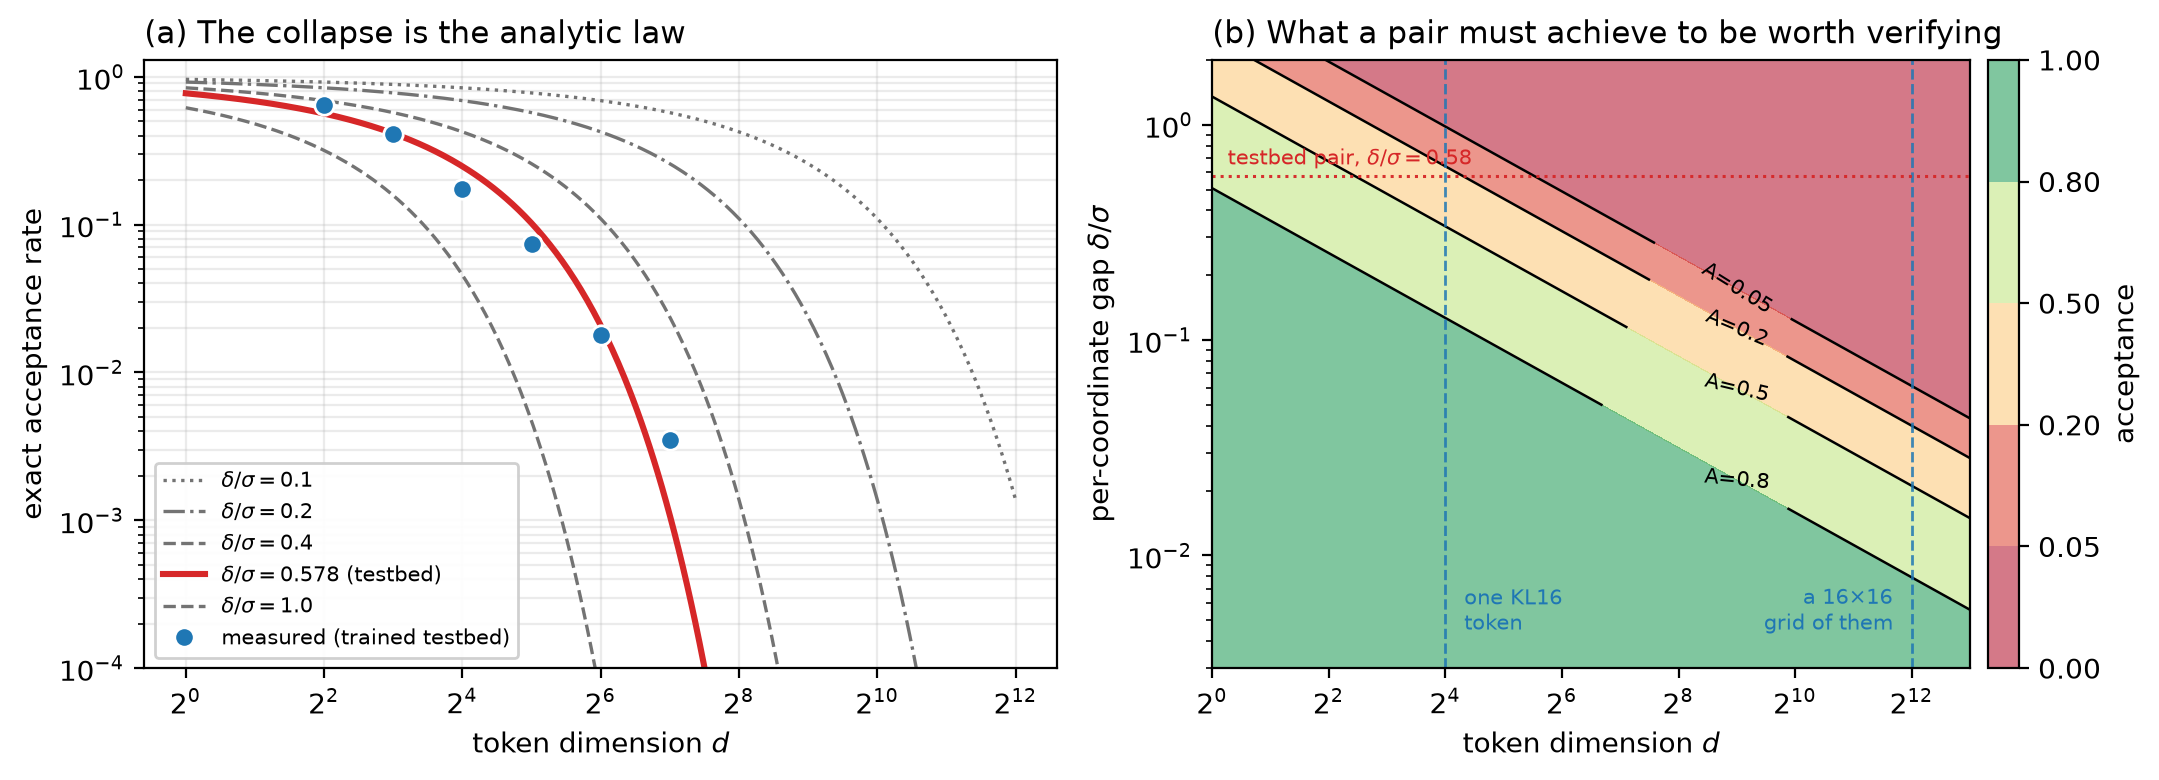
\includegraphics[width=0.86\textwidth]{figures/e08_feasibility.png}
\caption{\textbf{The collapse is an analytic law, and it has an engineering reading.}
\textbf{(a)} Exact acceptance against token dimension for shared-covariance Gaussians at several
fixed per-coordinate gaps, with the trained testbed's six measured rates overlaid. The measurements
track the $\delta/\sigma = 0.578$ curve they should, so the sweep samples a law rather than an
artefact of one architecture, and the law continues past the widths we can train: at $\dd = 256$
acceptance is already below $10^{-5}$. \textbf{(b)} The same statement as a design constraint.
Contours of acceptance over token dimension and per-coordinate disagreement are lines of
$\delta\sqrt{\dd} = \text{const}$, so on log--log axes they have slope $-1/2$ and every doubling of
the token width costs a factor $\sqrt2$ in the agreement a pair must reach. One KL16 token
($\dd{=}16$) tolerates a gap of $0.34\sigma$ at acceptance $0.5$; the $16\times16$ grid of them that
makes up an image ($\dd{=}4096$) tolerates $0.021\sigma$.}
\label{fig:feasibility}
\end{figure}


\section{Projection Redistributes the Divergence It Cannot Reduce}
\label{sec:conservation}

\subsection{Projected verification and its null control}

Let $A \in \R^{\kk \times \dd}$ have orthonormal rows and verify $s = Ax$: accept with probability
$\min\{1, p_A(s)/q_A(s)\}$ for pushforwards $p_A, q_A$. For a Gaussian mixture the pushforward is
again one, with means $A\mu$ and \emph{full} covariances $A\operatorname{diag}(\sigma^2)A^\top$, which
we compute exactly rather than approximate.

Two facts make the comparison across rules well posed. First, when $\kk = \dd$ the map is a bijection
with unit Jacobian and the projected ratio equals the exact one identically, a property we use as a
correctness test. Second, and more useful:

\begin{proposition}[Row-space invariance]
\label{prop:rowspace}
For any invertible $Q \in \R^{\kk \times \kk}$, the statistics $Ax$ and $QAx$ induce the same
acceptance probability at every $x$.
\end{proposition}

The Jacobian $|\det Q|$ multiplies numerator and denominator alike and cancels
(Appendix~\ref{app:proofs}). Such a rule is therefore not a matrix but a \emph{choice of
$\kk$-dimensional subspace}: rules reaching the same subspace by different constructions are one rule.

Before asking which subspace is best, one must ask whether the choice matters at all. Any dimension
reduction raises acceptance for free reasons (the $h^\dd$ scaling \citet{fearnhead2012constructing}
identify in ABC), so a structureless projection is the mandatory null control. Across the full sweep,
acceptance under random subspaces is very nearly a function of the verified dimension $\kk$
\emph{alone}: at $\kk=4$ the mean rate is $0.624$ over $\dd \in \{4,\dots,128\}$ with a coefficient of
variation of $2.5\%$, and over $\kk \in \{1,\dots,32\}$ that variation stays between $1.3\%$ and
$12.3\%$. Proposition~\ref{prop:random} below derives this rather than leaving it as an observation. A
random projection lifts acceptance at $\dd{=}128$ from $0.0035$ to $0.64$, a $180\times$ gain, while
knowing nothing about the model. Acceptance alone therefore cannot tell a good statistic from a
worthless one, and the question moves entirely to what each rule \emph{costs}.

\subsection{What projection can and cannot do}

The first fact costs no assumptions at all. Verifying a statistic and letting the complement through
does not destroy any divergence; it moves divergence out of the test's view.

\begin{proposition}[Divergence is split, never reduced]
\label{prop:split}
Let $p, q$ be densities on $\R^\dd$ and let $R = [A; A_\perp]$ be orthogonal, so $x \mapsto (s,u) =
(Ax, A_\perp x)$ is a bijection. Then
\begin{equation}
\KL(p \,\|\, q) \;=\; \underbrace{\KL(p_A \,\|\, q_A)}_{\text{seen by the test}}
\;+\; \underbrace{\E_{p_A}\!\left[\KL\bigl(p(u \mid s) \,\|\, q(u \mid s)\bigr)\right]}_{\text{escapes the test}},
\label{eq:split}
\end{equation}
and the left-hand side does not depend on $A$.
\end{proposition}

This is the chain rule for KL applied to a bijection (Appendix~\ref{app:proofs}); it needs no
Gaussian assumption, no shared covariance, and no structure in $\delta$. It already says the thing
the design intuition gets wrong. A verifier chooses $A$, and thereby chooses how to \emph{divide} a
total it cannot alter; acceptance is bought from the first term and paid for in the second.

Adding shared-covariance Gaussians turns the split into a curve with a closed form.

\begin{proposition}[Gaussian conservation and the closed-form frontier]
\label{prop:conservation}
Let $p = \mathcal{N}(\mu_p, \sigma^2 I)$ and $q = \mathcal{N}(\mu_q, \sigma^2 I)$ on $\R^\dd$ with
$\delta = \mu_p - \mu_q$, and let $A \in \R^{\kk\times\dd}$ have orthonormal rows. The conditional
term in Eq.~\ref{eq:split} is then the marginal $\KL(p_{A_\perp} \| q_{A_\perp})$, and
\begin{equation}
\KL(p_A \,\|\, q_A) \;+\; \KL(p_{A_\perp} \,\|\, q_{A_\perp}) \;=\; \KL(p \,\|\, q)
\;=\; \frac{\|\delta\|^2}{2\sigma^2}.
\label{eq:conservation}
\end{equation}
Moreover the projected acceptance rate is $2 - 2\Phi\!\left(\|A\delta\|/2\sigma\right)$, a function of
$\|A\delta\|^2$ alone.
\end{proposition}

% The conservation identity, drawn three ways: the geometry that produces it, the two things the two
% halves control, and the budget picture that makes the corollary obvious. Laid out as three columns
% so the figure stays short enough for the main text's page budget.
\begin{figure}[t]
\centering
\resizebox{0.90\textwidth}{!}{%
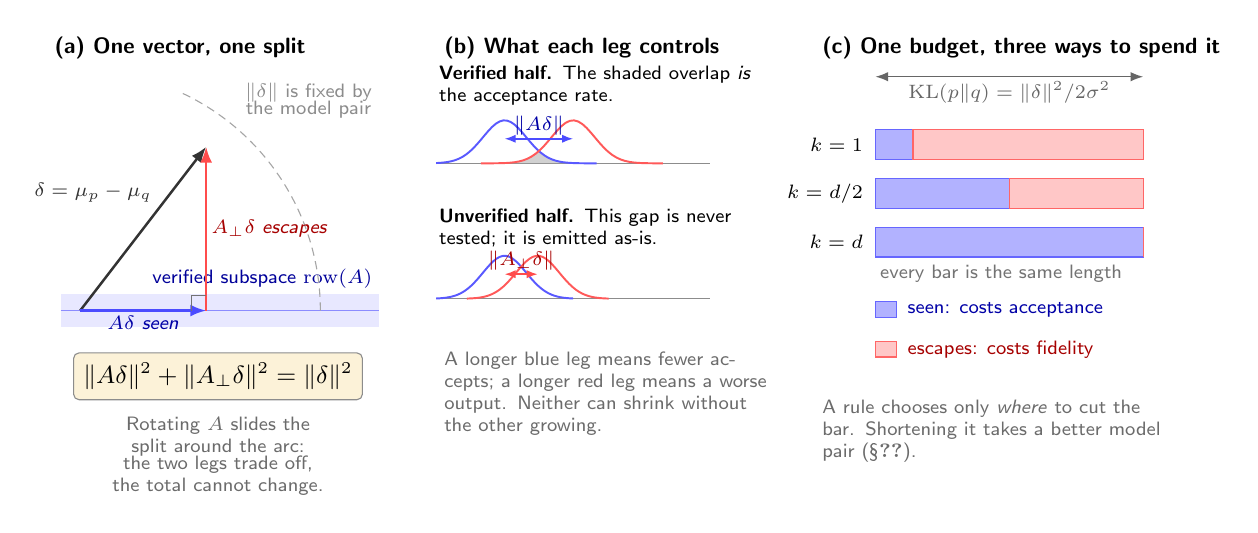
\begin{tikzpicture}[
  font=\sffamily\small,
  hd/.style   = {font=\sffamily\bfseries\footnotesize, anchor=north west},
  note/.style = {font=\sffamily\scriptsize, text=black!58, align=center},
  lbl/.style  = {font=\sffamily\scriptsize, inner sep=1.5pt},
  vec/.style  = {-{Latex[length=2.0mm]}, line width=0.9pt},
]

%=================== (a) the Pythagorean split ===================
\node[hd] at (0,4.55) {(a) One vector, one split};

\coordinate (O) at (0.45,0.95);
% the verified subspace, drawn as a band through the origin
\fill[blue!9] (0.20,0.74) rectangle (4.25,1.16);
\draw[blue!45, line width=0.5pt] (0.20,0.95) -- (4.25,0.95);
\node[lbl, text=blue!60!black, anchor=east] at (4.22,1.36) {verified subspace $\operatorname{row}(A)$};

% arc of fixed radius: the total is the thing that does not move
\draw[densely dashed, black!35] ($(O)+(0:3.05)$) arc (0:66:3.05);
\node[note, anchor=west, text=black!45] at (2.42,3.62) {$\|\delta\|$ is fixed by\\[-2pt] the model pair};

\coordinate (D) at (2.05,3.03);
\coordinate (P) at (2.05,0.95);
\draw[vec, black!80] (O) -- (D) node[pos=0.62, above left, lbl, inner sep=2pt]{$\delta=\mu_p-\mu_q$};
\draw[vec, blue!70]  (O) -- (P) node[pos=0.5, below, lbl, text=blue!65!black]{$A\delta$ \emph{seen}};
\draw[vec, red!70]   (P) -- (D) node[pos=0.5, right, lbl, text=red!65!black]{$A_\perp\delta$ \emph{escapes}};
\draw[black!55, line width=0.4pt] ($(P)+(-0.19,0)$) -- ++(0,0.19) -- ++(0.19,0);

\node[draw=black!45, rounded corners=2pt, fill=amber!18, inner sep=3.5pt, anchor=north, font=\small]
  at (2.2,0.42) {$\|A\delta\|^{2} + \|A_\perp\delta\|^{2} = \|\delta\|^{2}$};
\node[note, anchor=north, text width=4.6cm] at (2.2,-0.28)
  {Rotating $A$ slides the split around the arc:\\[-2pt]
   the two legs trade off, the total cannot change.};

%=================== (b) what each leg controls ===================
\node[hd] at (4.95,4.55) {(b) What each leg controls};

\node[lbl, anchor=north west, text width=4.25cm] at (4.95,4.12)
  {\textbf{Verified half.} The shaded overlap \emph{is} the acceptance rate.};

% -- verified half: overlap is the acceptance rate
\begin{scope}[shift={(5.15,2.82)}, xscale=0.60, yscale=0.52]
  \draw[black!45, line width=0.4pt] (-0.3,0) -- (5.5,0);
  % overlap = min of the two densities, drawn as two half-regions meeting at the crossing point
  \fill[black!30, opacity=0.6]
    plot[domain=-0.30:1.875,samples=32] (\x,{1.05*exp(-(\x-2.6)*(\x-2.6)/0.42)}) --
    plot[domain=1.875:4.50,samples=32] (\x,{1.05*exp(-(\x-1.15)*(\x-1.15)/0.42)}) --
    (4.50,0) -- (-0.30,0) -- cycle;
  \draw[blue!65, line width=0.7pt] plot[domain=-0.30:3.10,samples=44]
       (\x,{1.05*exp(-(\x-1.15)*(\x-1.15)/0.42)});
  \draw[red!65, line width=0.7pt]  plot[domain=0.65:4.50,samples=44]
       (\x,{1.05*exp(-(\x-2.6)*(\x-2.6)/0.42)});
  % arrow set between the peaks rather than above them, which keeps the column short
  \draw[{Latex[length=1.4mm]}-{Latex[length=1.4mm]}, blue!70, line width=0.6pt]
       (1.15,0.60) -- node[lbl, above, text=blue!65!black, inner sep=1pt]{$\|A\delta\|$} (2.6,0.60);
\end{scope}
\node[lbl, anchor=north west, text width=4.25cm] at (4.95,2.30)
  {\textbf{Unverified half.} This gap is never tested; it is emitted as-is.};

% -- unverified half: leaks
\begin{scope}[shift={(5.15,1.10)}, xscale=0.60, yscale=0.52]
  \draw[black!45, line width=0.4pt] (-0.3,0) -- (5.5,0);
  \draw[blue!65, line width=0.7pt] plot[domain=-0.30:2.60,samples=44]
       (\x,{1.05*exp(-(\x-1.15)*(\x-1.15)/0.42)});
  \draw[red!65, line width=0.7pt]  plot[domain=0.35:3.35,samples=44]
       (\x,{1.05*exp(-(\x-1.85)*(\x-1.85)/0.42)});
  \draw[{Latex[length=1.4mm]}-{Latex[length=1.4mm]}, red!70, line width=0.6pt]
       (1.15,0.60) -- node[lbl, above, text=red!65!black, inner sep=1pt]{$\|A_\perp\delta\|$} (1.85,0.60);
\end{scope}
\node[note, anchor=north west, text width=4.25cm, align=left] at (4.95,0.55)
  {A longer blue leg means fewer accepts; a longer red leg means a worse output. Neither can shrink
   without the other growing.};

%=================== (c) the budget ===================
\node[hd] at (9.75,4.55) {(c) One budget, three ways to spend it};

\draw[{Latex[length=1.6mm]}-{Latex[length=1.6mm]}, black!60, line width=0.5pt]
  (10.55,3.92) -- node[lbl, below, inner sep=1.5pt]{$\KL(p\|q)=\|\delta\|^{2}/2\sigma^{2}$} (13.95,3.92);

\foreach \i/\k/\frac in {0/{$\kk=1$}/0.14, 1/{$\kk=\dd/2$}/0.50, 2/{$\kk=\dd$}/1.00} {
  \pgfmathsetmacro{\yy}{3.06 - \i*0.62}
  \pgfmathsetmacro{\split}{10.55 + \frac*3.40}
  \node[lbl, anchor=east] at (10.45,\yy) {\k};
  \fill[blue!30, draw=blue!60, line width=0.4pt] (10.55,\yy-0.19) rectangle (\split,\yy+0.19);
  \fill[red!22,  draw=red!60,  line width=0.4pt] (\split,\yy-0.19) rectangle (13.95,\yy+0.19);
}
\node[lbl, anchor=west, text=black!55] at (10.55,1.42) {every bar is the same length};

\fill[blue!30, draw=blue!60, line width=0.4pt] (10.55,0.86) rectangle (10.82,1.06);
\node[lbl, anchor=west, text=blue!65!black] at (10.90,0.96) {seen: costs acceptance};
\fill[red!22,  draw=red!60,  line width=0.4pt] (10.55,0.36) rectangle (10.82,0.56);
\node[lbl, anchor=west, text=red!65!black]  at (10.90,0.46) {escapes: costs fidelity};

\node[note, anchor=north west, text width=4.3cm, align=left] at (9.75,-0.06)
  {A rule chooses only \emph{where} to cut the bar. Shortening it takes a better
   model pair (\S\ref{sec:moving}).};

\end{tikzpicture}}
\caption{\textbf{Why projected verification cannot help.}
\textbf{(a)}~For a shared-covariance Gaussian pair the whole problem is one vector, the mean gap
$\delta$, and an orthonormal $A$ splits it into a part the test sees and a part orthogonal to the
test. Because the split is orthogonal, Pythagoras fixes the sum.
\textbf{(b)}~Neither leg is abstract: the one the test sees sets the overlap of the projected
densities, which \emph{is} the acceptance rate, and the one that escapes is emitted unchecked, which
\emph{is} the fidelity cost.
\textbf{(c)}~So the divergence is a fixed budget and the rank $\kk$ only picks where to spend it. No
choice shortens the bar, which is what confines all five rules to one measured curve
(Figure~\ref{fig:onefrontier}) and why \S\ref{sec:moving} attacks the bar's length instead.}
\label{fig:conservation}
\end{figure}


Here the split is the Pythagorean identity $\|A\delta\|^2 + \|A_\perp\delta\|^2 = \|\delta\|^2$
(Appendix~\ref{app:proofs}), drawn in Figure~\ref{fig:conservation}: what the statistic \emph{sees}
sets acceptance, what \emph{escapes} it sets the fidelity cost, and their sum is pinned. Because both
coordinates of the trade-off are functions of the single quantity $\|A\delta\|^2$, eliminating it
leaves one curve.

\begin{corollary}[One frontier]
\label{cor:frontier}
Under Proposition~\ref{prop:conservation}, every orthonormal statistic of every rank lies on a single
acceptance--fidelity frontier determined by $\|\delta\|/\sigma$. A subspace rule selects a
\emph{point} on that frontier; it cannot move the frontier itself.
\end{corollary}

The distinction matters, because subspace choice emphatically does change acceptance: at
$\dd{=}128, \kk{=}16$ our rules span $0.018$ to $0.550$, a $30\times$ range. What Corollary~\ref{cor:frontier}
denies is not that rules differ but that any of them buys acceptance more cheaply than another. The
anti-control is not bad luck; it sits at the high-acceptance, high-leakage end of the same curve.

\paragraph{Random subspaces at finite $\dd$.} The null control's behaviour follows from the same
picture, and deriving it properly is worth the half page because the obvious argument is invalid.
One cannot substitute $\E\|A\delta\|^2 = (\kk/\dd)\|\delta\|^2$ into the acceptance formula, since
$z \mapsto 2 - 2\Phi(\sqrt{z}/2\sigma)$ is nonlinear and $\E[f(Z)] \ne f(\E Z)$; on our sweep that
step errs by $2.8$--$8.8\%$. The correct statement uses the exact law of the captured fraction.

\begin{proposition}[Random subspaces]
\label{prop:random}
For $A$ uniform on the Stiefel manifold, $Z = \|A\delta\|^2/\|\delta\|^2 \sim
\operatorname{Beta}(\kk/2, (\dd-\kk)/2)$, so the expected acceptance is
$\E_Z\bigl[2 - 2\Phi(M\sqrt{Z}/2)\bigr]$ with $M = \|\delta\|/\sigma$. If the per-coordinate gap is
held fixed, so that $M = c\sqrt{\dd}$, then $M^2 Z \Rightarrow c^2 \chi^2_\kk$ as $\dd \to \infty$
with $\kk$ fixed, a limit free of $\dd$.
\end{proposition}

So acceptance under a random subspace is asymptotically a function of $\kk$ alone, with an $O(1/\dd)$
correction rather than by coincidence. Evaluating the exact Beta expression over $\dd \in \{16,\dots,4096\}$
gives a coefficient of variation across dimensions of $0.15\%$ at $\kk{=}1$ and $1.7\%$ at $\kk{=}32$,
which is the analytic counterpart of the $1.3\%$--$12.3\%$ we measure on trained models.

\paragraph{Why transform coding does not transfer.} The intuition Eq.~\ref{eq:conservation} overturns
is a good one, so it is worth saying exactly where it breaks. Transform coding rests on \emph{energy
compaction} \citep{goyal2001transform}: natural images are smooth, the DCT packs nearly all of their
energy into a few low-frequency coefficients, and a codec discards the rest and still reconstructs a
convincing picture. The transform does not create that concentration, it reveals it.

Verification asks the same question about a different object. What must be checked is not the token
but the discrepancy $\delta = \mu_p - \mu_q$, and Parseval applies to $\delta$ exactly as it applies
to an image, which is precisely the difficulty: an orthonormal change of basis can only
\emph{redistribute} $\delta$ between the coefficients we inspect and the ones we do not. For
compression the invariance is harmless because the payoff comes from concentration that is already
there. For verification there is no reason to expect any: two separately trained networks disagree
wherever they happen to disagree, and neither training objective aligns that disagreement with the
low-frequency band or any other nameable subspace. The asymmetry is informational. A codec picks its
basis knowing the statistics of what it will encode; a verifier must pick one before knowing where
the two models will differ, and Eq.~\ref{eq:conservation} guarantees that whatever goes unchecked is
emitted in full.

\subsection{Testing the prediction against five subspace rules}
\label{sec:metric}

Proposition~\ref{prop:conservation} is exact only for shared-covariance Gaussians. Our models are
Gaussian mixtures with heteroscedastic components, so the identity is an approximation and the
question is whether it survives. We test it with five rules spanning the space of plausible design
choices, all at matched $\kk$, all reduced to orthonormal bases by Proposition~\ref{prop:rowspace}.
Two of them anchor the comparison: \textbf{dct-low} is the transform-coding rule of \S\ref{sec:intro},
the one an image-processing practitioner would reach for first, and \textbf{signal-bottom} is its
opposite, built to be as bad as we could make it. If the choice of subspace is a design lever at all,
these two must be far apart.

\begin{itemize}
\itemsep1pt
\item \textbf{random}: uniform on the Stiefel manifold. The null control.
\item \textbf{pca}: top-$\kk$ principal directions of the token distribution. Knows the data.
\item \textbf{signal-top}: top-$\kk$ eigenvectors of $\E[J^\top J]$ for the decoder Jacobian $J$:
the latent directions that move the reconstructed waveform most. Knows the decoder.
\item \textbf{dct-low}: the transform-coding rule. Restrict the previous rule to the low-frequency DCT
band, i.e.\ take top eigenvectors of $\E[J^\top C^\top C J]$ for a band selector $C$. This verifies
the latent directions that move the reconstruction most \emph{within the band a codec would keep},
which is the speculative-decoding translation of what JPEG does. Composing the DCT with the Jacobian
keeps the statistic linear, so the pushforward stays Gaussian and the test stays exact.
\item \textbf{signal-bottom}: the adversarial anti-control: verify the directions that matter
\emph{least}. If the choice of subspace matters at all, this must be clearly worst.
\end{itemize}

\paragraph{A fidelity metric that cannot be gamed.} Our first attempt failed instructively. The
obvious signal-domain metric is excess squared error: decode the emitted tokens, compare against the
real window, and subtract what a genuine target draw would incur. Under it \emph{every} rule scored
\emph{negative} excess distortion and the anti-control scored best of all, because the draft is the
smaller model, its samples sit nearer the conditional mean, and squared error against a single
reference rewards exactly that variance shrinkage. A rule emitting the conditional mean would win it
outright while being a useless sampler. We therefore report two costs without this defect
(Appendix~\ref{app:metric}):
\begin{itemize}
\itemsep1pt
\item \textbf{Excess NLL under the target}, $\E_{\tilde p}[-\log p] - \E_{p}[-\log p]$, in nats per
token. This is a zero-anchored cross-entropy discrepancy, not a divergence: it vanishes when
$\tilde p = p$, but it is neither $\KL(\tilde p \| p)$ nor guaranteed non-negative, so we read its
\emph{sign} as diagnostic and its magnitude only in comparison across rules at matched acceptance.
\item \textbf{Signal-domain energy distance}, $2\E\|X-Y\| - \E\|X-X'\| - \E\|Y-Y'\|$ between decoded
emitted waveforms $X,X'$ and decoded target waveforms $Y,Y'$ under matched conditioning. It is zero
exactly when the decoded distributions agree, and the $-\E\|X-X'\|$ term \emph{penalises} the mode
collapse that squared error rewards.
\end{itemize}
Exact verification anchors both at zero at every dimension: the excess NLL of the exact rule is
within $1.2$ standard errors of zero for all six values of $\dd$ (largest deviation $+0.188 \pm 0.190$
nats at $\dd{=}128$), and the residual sampler converges on $100.0\%$ of rejections throughout.

\begin{table}[t]
\centering
\small
\begin{tabular}{lcccc}
\toprule
$\dd$ & cost range spanned & median deviation & max deviation & \textbf{max as \% of range} \\
 & (nats/token) & from one curve & from one curve & \\
\midrule
4   & 0.240  & 0.027 & 0.038 & \cgood{10}{15.9\%} \\
8   & 1.560  & 0.017 & 0.112 & \cgood{22}{7.2\%} \\
16  & 5.768  & 0.050 & 0.356 & \cgood{25}{6.2\%} \\
32  & 11.341 & 0.331 & 0.950 & \cgood{19}{8.4\%} \\
64  & 26.305 & 0.616 & 1.476 & \cgood{29}{5.6\%} \\
128 & \textbf{48.016} & 0.777 & 1.933 & \cgood{40}{$\best{4.0\%}$} \\
\bottomrule
\end{tabular}
\caption{Five subspace rules, one frontier, across a $32\times$ range of token dimension. Each rule's
cost is compared against the random-projection curve interpolated to the \emph{same acceptance}.
Costs vary over $48$ nats at $\dd{=}128$, yet no rule departs from a single curve by more than
$\best{4.0\%}$ of that range, and the margin \emph{tightens} as $\dd$ grows. Energy-distance figures
tell the same story and are in Appendix~\ref{app:results}.
\emph{Shading.} Deeper green is a \emph{smaller} departure, so the column darkening downwards is the
evidence strengthening with dimension.}
\label{tab:collapse}
\end{table}

\begin{figure}[t]
\centering
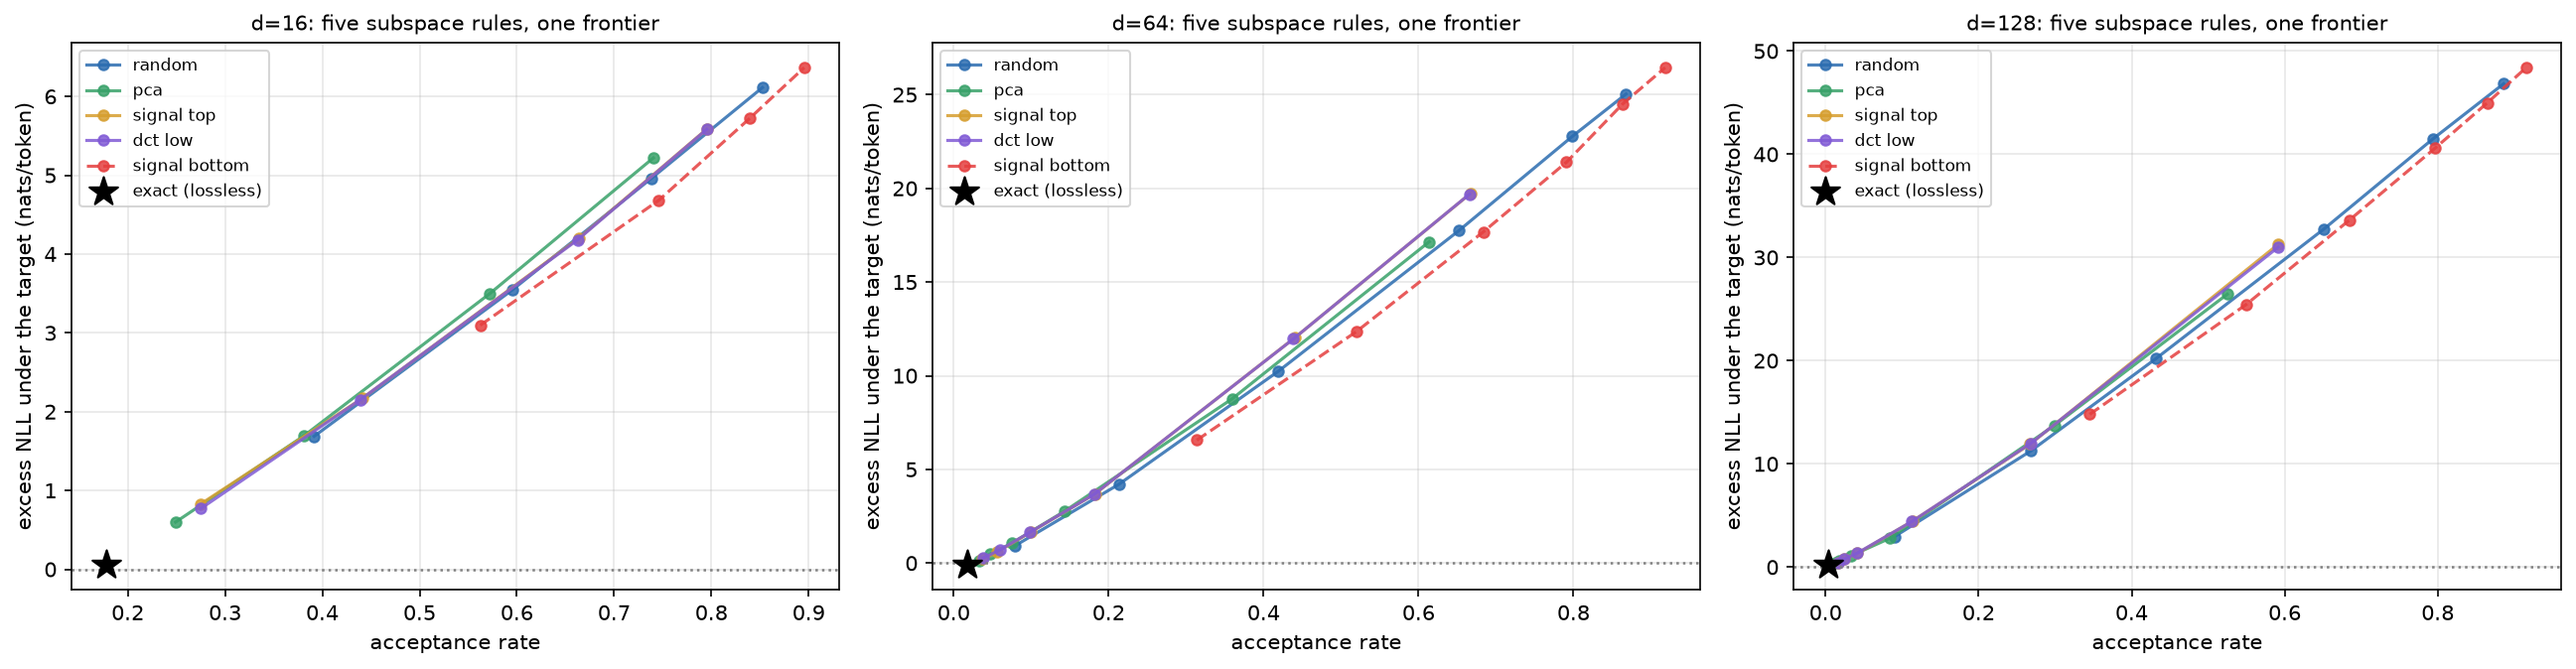
\includegraphics[width=0.77\textwidth]{figures/e12b_collapse_compact_gpu.png}
\caption{\textbf{Five subspace rules, one frontier.} Excess NLL against acceptance for all five
rules and every $\kk$; a point's position along a curve is set by $\kk$, and the question is whether
the curves differ. They do not: the rules span $48$ nats at $\dd{=}128$ and depart from one another
by at most $\best{4.0\%}$ of that range. The anti-control (red, dashed), which verifies the \emph{least}
important directions, is not separated from the rule built with full knowledge of the decoder. The
black star marks exact verification, which is lossless and anchors the metric at zero. The
signal-domain energy distance gives the same picture and is shown in
Figure~\ref{fig:onefrontier-full}.}
\label{fig:onefrontier}
\end{figure}

\paragraph{Result.} Table~\ref{tab:collapse} and Figure~\ref{fig:onefrontier} report the test over
six token dimensions from $4$ to $128$. For each structured point we
interpolate the random-projection curve to the same acceptance and record the difference; we never
extrapolate, so every comparison is against a baseline actually observed at that rate. At $\dd = 128$
the cost of these rules ranges over $48.0$ nats, and the largest departure from a single curve is
$1.93$ nats, or $\best{4.0\%}$ of the range; at $\dd = 64$ the figures are $26.3$ nats and $5.6\%$.
The relative margin does not loosen as the token grows, it tightens, so the collapse is sharpest in
precisely the regime where escaping it would be worth the most. The energy
distance tells the same story with a larger relative tolerance, driven by its higher variance.

Three details make this more than a null result. First, the \emph{ordering} is not stable: the
anti-control ranks \emph{best} at the three largest dimensions ($1.50$ nats below the random curve at
$\dd{=}128$, $\kk{=}16$) while the decoder-Jacobian rule ranks worst there. Once acceptance is held
fixed, a rule designed to be maximally stupid is indistinguishable from one built with full knowledge
of the decoder. Second, the rules differ enormously at matched $\kk$: at $\dd{=}128,\kk{=}16$
acceptance spans $0.018$ (pca) to $0.550$ (anti-control), a $30\times$ range, so these are genuinely
different rules landing on the same curve, which is the distinction
Corollary~\ref{cor:frontier} draws between choosing a point and moving the frontier.

Third, and this is the one that matters for an image pipeline, the transform-coding rule is not a
strawman and still gains nothing. At $\dd{=}128, \kk{=}16$, \textbf{dct-low} and the anti-control are
about as different as two rules can be, separated by a factor of $22$ in acceptance ($0.025$ against
$0.550$) and by $24.7$ nats in cost, and yet both sit within $4.0\%$ of the same curve. Nor is
\textbf{dct-low} weak on its own terms: it tracks \textbf{signal-top} to within a few thousandths in
every cell of the appendix table, so the low-frequency band and the directions the decoder is most
sensitive to are very nearly the same subspace. The JPEG heuristic identifies the perceptually
important directions correctly, and identifying them correctly is what buys nothing.

\section{Is There a Perceptual Band to Keep?}
\label{sec:kl16}

Corollary~\ref{cor:frontier} says that identifying the perceptually important directions cannot move
the frontier. It is worth asking the prior question as well, on the actual image model rather than
the testbed: are there such directions to identify? Projected verification is motivated by the
picture in which a handful of latent directions dominate what the viewer sees and the rest are slack.
If the KL16 decoder were built that way, the transform-coding intuition would at least be attacking a
real structure. We measured whether it is, and found no sign of one.

\paragraph{What we measured.} For the frozen KL16 autoencoder that MAR uses, we compute the decoder's
local Jacobian spectrum at four ImageNet latents, obtained by re-encoding MAR-B's own samples so they
sit where the sampler operates. The latent is $16 \times 16 \times 16$, so the decoder maps $4096$
numbers to a $256 \times 256$ image; we recover the top $64$ singular values by randomised SVD with
matrix-free Jacobian-vector and vector-Jacobian products. These are perceptual gains: $\sigma_i$ is
how far the decoded image moves per unit movement along latent direction $i$. Effective rank, the
exponentiated entropy of the normalised spectrum, is $64$ for a flat spectrum and $1$ if one direction
dominates.

\begin{table}[t]
\centering
\small
\begin{tabular}{lccccc}
\toprule
latent & anisotropy (top-$64$) & effective rank (of $64$) & $\sigma_{\max}$ & $\sigma_{\min}$ \\
\midrule
0 & 4.08 & 60.69 & 23.61 & 5.79 \\
1 & 3.05 & 61.44 & 15.99 & 5.25 \\
2 & 3.58 & 60.56 & 19.54 & 5.46 \\
3 & 2.60 & 61.75 & 47.38 & 18.24 \\
\midrule
median & $\best{3.31}$ & $\best{61.06}$ & & \\
\bottomrule
\end{tabular}
\caption{Among the directions we can measure, the KL16 decoder is close to isotropic. Across the top
$64$ of $4096$ latent directions the perceptual gain varies by only $3.31\times$ and the effective
rank is $61$ of $64$, so those directions carry near-equal response rather than a few dominating. The
linearisation is trustworthy at the scale a verifier works in: measured finite-difference gain agrees
with the Jacobian's prediction to a median relative error of $0.054$ (max $0.076$) at $\epsilon =
10^{-2}$.}
\label{tab:kl16}
\end{table}

\paragraph{Result.} Table~\ref{tab:kl16} reports the spectrum and Figure~\ref{fig:kl16} sets it
against the DCT spectrum of the very same images. Within a latent, the decoder is close to isotropic
over the directions we can resolve: gain varies by only $3.31\times$ across the top $64$, and the
effective rank is $61.06$ of $64$, meaning those directions carry nearly equal perceptual weight
rather than a few carrying most of it. The comparison in Figure~\ref{fig:kl16}(a) is the sharpest way
to see it. Sorted and normalised the same way, the image's DCT coefficients have fallen to $1.5\%$ of
the leading coefficient by rank $64$, while the decoder's singular values are still at $30\%$, a
decay roughly $20\times$ shallower. This is the empirical counterpart of the argument in
\S\ref{sec:conservation}: a codec can discard high frequencies because a natural image's energy
spectrum really does collapse, and over the directions we can measure the KL16 decoder's sensitivity
spectrum does not. We state this as an absence of evidence rather than evidence of absence. What the
measurement establishes is that there is \emph{no compact perceptual band among the top $64$ of
$4096$ decoder-sensitive directions}; the remaining $4032$ are uncharacterised, and a strongly
attenuated tail there would not show up in this experiment.

\begin{figure}[t]
\centering
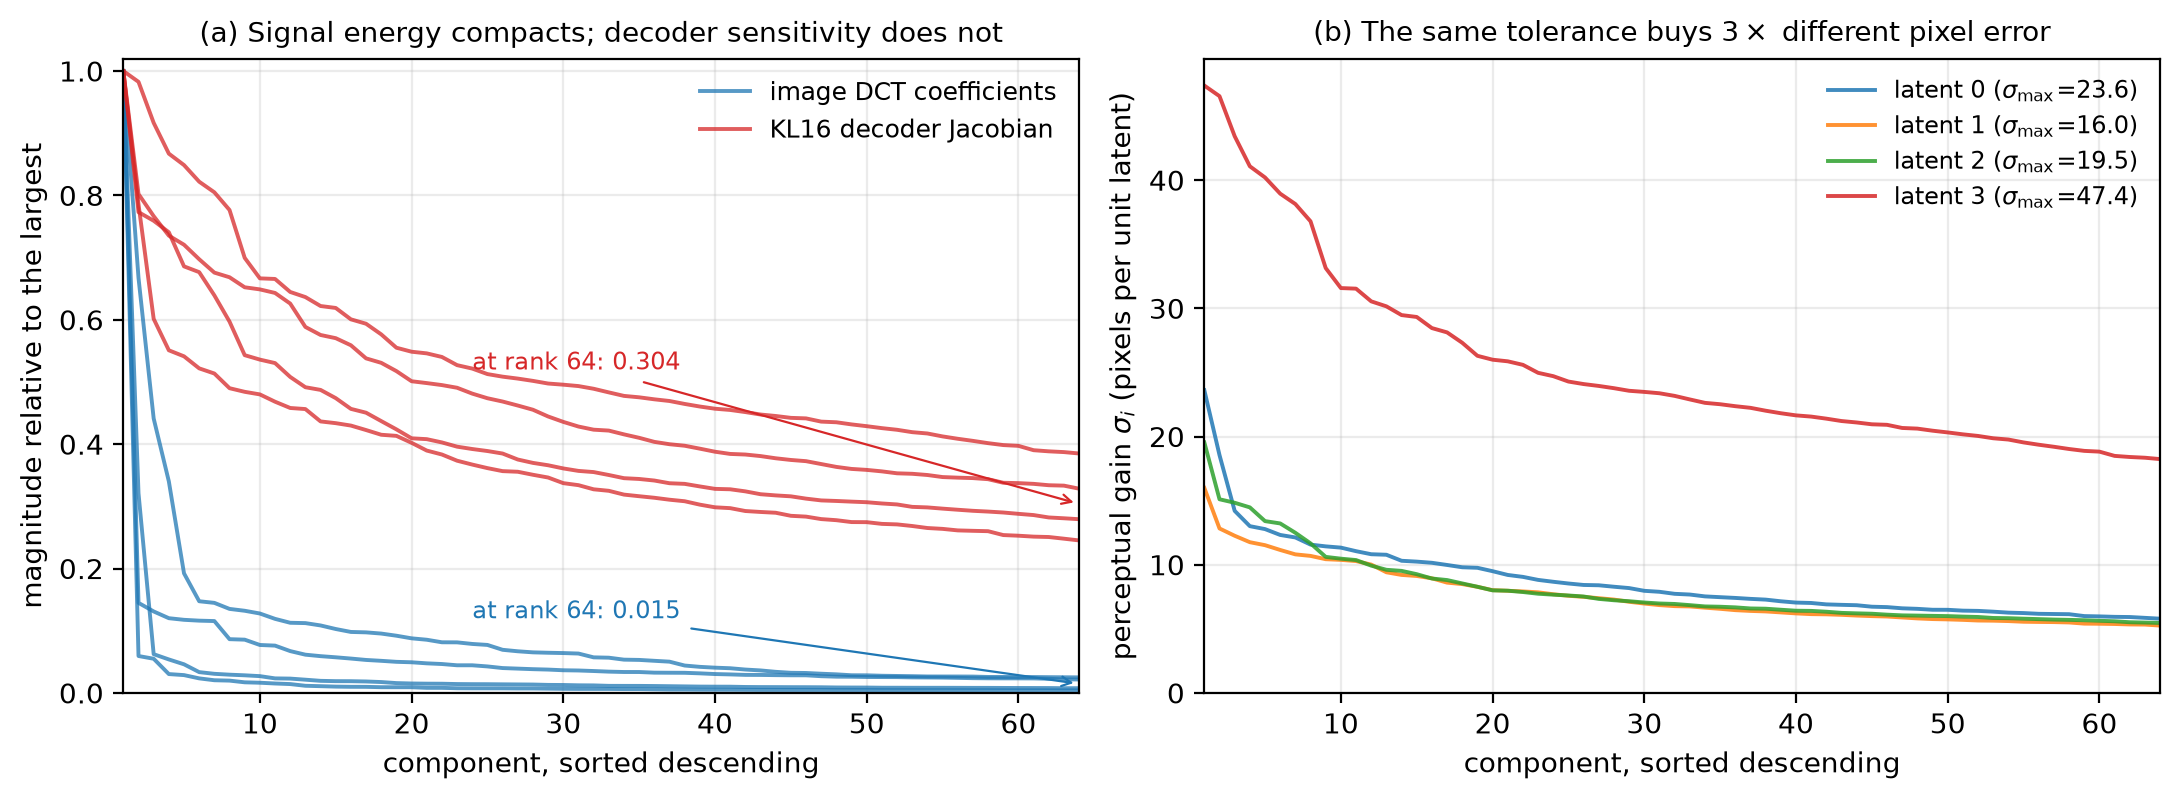
\includegraphics[width=0.75\textwidth]{figures/e05_kl16_spectrum.png}
\caption{\textbf{No compact band among the directions we can measure.} Two spectra of the same four ImageNet
samples, each sorted descending and truncated to the top $64$ components so that they are directly
comparable. \textbf{(a)} The $2$D DCT coefficients of the decoded image (blue) fall to $1.5\%$ of the
leading coefficient by rank $64$: this steep decay is the premise transform coding runs on, and it is
why JPEG can throw the tail away. The singular values of the KL16 decoder's local Jacobian (red),
which measure how far the image moves per unit movement along each latent direction, are still at
$30\%$ at the same rank, a decay $20\times$ shallower. There is no small set of latent directions
carrying the perceptual content, so no compact band whose complement is cheap to leave unverified.
\textbf{(b)} The absolute gains, where a second problem appears: $\sigma_{\max}$ varies from $16.0$ to
$47.4$ \emph{between} images, so a fixed latent-space tolerance buys threefold different pixel error
depending on which image is being generated.}
\label{fig:kl16}
\end{figure}

\paragraph{What it does not say.} It does not measure where draft and target disagree, the quantity
Proposition~\ref{prop:conservation} governs; it measures only whether the decoder concentrates
perceptual response, and finds no sign that it does. The two arguments are complementary rather than
the same one twice. It also surfaces a problem the design question did not ask about:
$\sigma_{\max}$ ranges from $15.99$ to $47.38$ across the four images, so a latent-space tolerance
buys threefold different pixel error depending on which image is generated, and any risk guarantee
stated in latent space is marginal over images rather than conditional on one. Four latents is a
pilot, the between-image spread is what four samples estimate worst, randomised SVD recovers only the
top of the spectrum, and the latents are re-encoded MAR samples rather than photographs; the
conclusion we draw is correspondingly the absence of a band among the top $64$ directions rather than
its absence overall.

\section{Moving the Frontier Instead of Sliding Along It}
\label{sec:moving}

Corollary~\ref{cor:frontier} is negative about rules but constructive about targets. If the frontier
is fixed by $\|\delta\|/\sigma$, a property of the model \emph{pair}, the only way to improve the
acceptance--fidelity trade is to bring the pair closer together, which no verification rule can do
and training can. We test this by distilling the draft against the frozen target with a mode-covering
objective, minimising $\KL(p\|q)$ by drawing from the target and scoring those draws under the draft.
The direction matters: reverse KL would let the draft collapse onto one mode and still score well,
whereas mode-covering pressure puts mass wherever the target has it, which is what acceptance is
sensitive to.

\begin{table}[t]
\centering
\small
\begin{tabular}{lccccc}
\toprule
$\dd$ & acceptance before & acceptance after & gain & fidelity cost & projection cost for same rate \\
\midrule
4   & 0.6453 & \textbf{0.7198} & \cgood{12}{$\best{1.12\times}$} & $\best{0}$ \textbf{(exact)} & $0.188$ nats/token \\
8   & 0.4018 & \textbf{0.4728} & \cgood{15}{$\best{1.18\times}$} & $\best{0}$ \textbf{(exact)} & $0.321$ nats/token \\
16  & 0.1779 & \textbf{0.2507} & \cgood{20}{$\best{1.41\times}$} & $\best{0}$ \textbf{(exact)} & $0.613$ nats/token \\
32  & 0.0722 & \textbf{0.1084} & \cgood{23}{$\best{1.50\times}$} & $\best{0}$ \textbf{(exact)} & $0.390$ nats/token \\
64  & 0.0176 & \textbf{0.0459} & \cgood{32}{$\best{2.61\times}$} & $\best{0}$ \textbf{(exact)} & $0.366$ nats/token \\
128 & 0.0036 & \textbf{0.0208} & \cgood{44}{$\best{5.72\times}$} & $\best{0}$ \textbf{(exact)} & $0.739$ nats/token \\
\bottomrule
\end{tabular}
\caption{Distillation moves the frontier, and the gain \emph{grows} with the token dimension. Exact
verification is lossless at every stage, so the acceptance gain is free (\textbf{bold}). The last
column is what the projection frontier must spend in excess NLL to reach the same acceptance,
interpolated from the measured curve: distillation buys it for nothing, which no rule in
Table~\ref{tab:collapse} can do. $10{,}000$ steps per dimension, five stages.
\emph{Shading.} Green depth tracks the gain, so the deepening column \emph{is} the dimensional trend;
the fidelity column is identically zero and so is left unshaded.}
\label{tab:e14}
\end{table}

\begin{figure}[t]
\centering
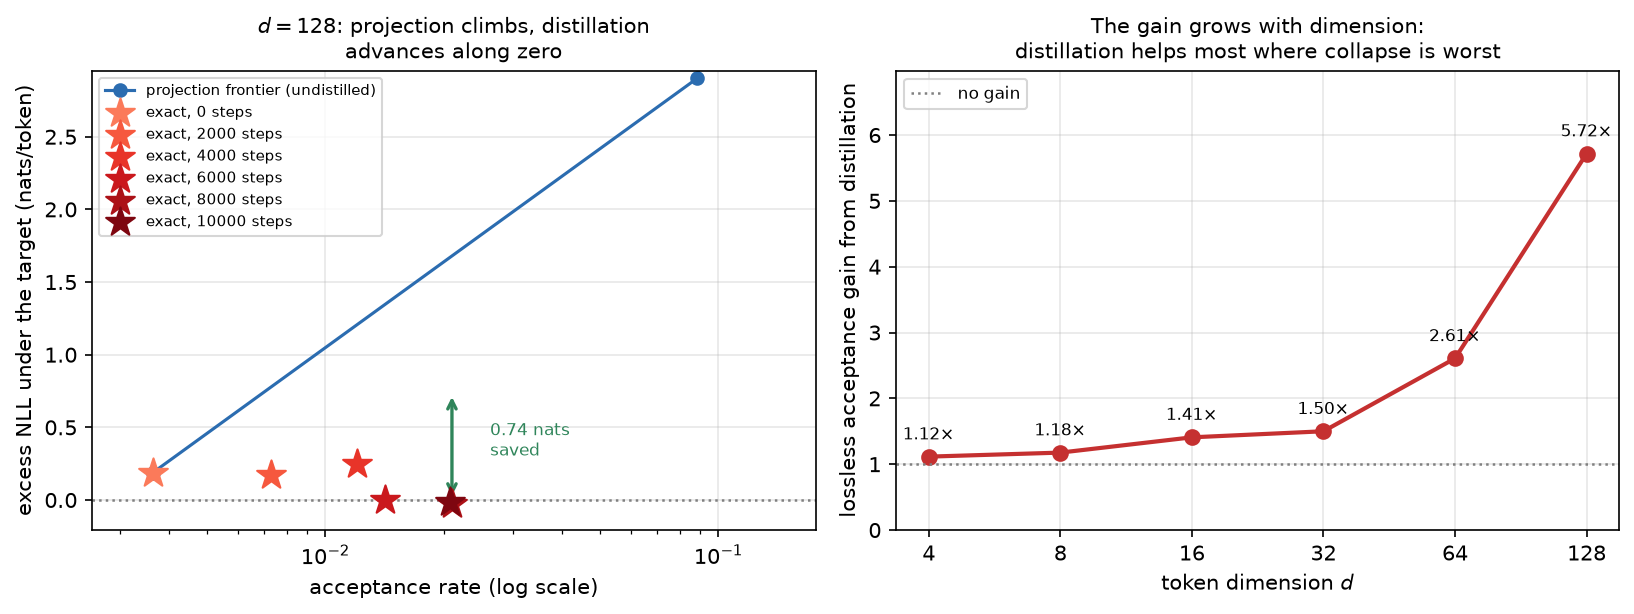
\includegraphics[width=0.68\textwidth]{figures/e14_alignment_gpu_headline.png}
\caption{\textbf{Projection slides along the frontier; distillation moves it.} \textbf{Left:} at
$\dd{=}128$, the blue curve is the projection frontier of the undistilled pair, and to gain
acceptance one must climb it, paying excess NLL. The stars are exact verification after successive
rounds of distillation: they advance \emph{rightwards along zero}, gaining acceptance at no fidelity
cost, which is a direction the frontier does not offer. The arrow marks the $0.74$ nats the frontier
charges for the rate distillation reached for free. \textbf{Right:} the gain is not a fixed bonus.
It grows monotonically with $\dd$, from $1.12\times$ to $\best{5.72\times}$, so the one intervention
that works helps most exactly where the collapse of \S\ref{sec:collapse} bites hardest. This is the
constructive content of Corollary~\ref{cor:frontier}: the curve is a property of the model pair, so
only changing the pair can move it.}
\label{fig:moving}
\end{figure}

Table~\ref{tab:e14} and Figure~\ref{fig:moving} show the effect after $10{,}000$ distillation steps at
each of six token dimensions. Acceptance rises at every one while the rule stays exact and therefore
lossless: the measured excess NLL sits within $1.2$ standard errors of zero throughout, and the
residual sampler converges on every rejection. The same acceptance by projection would cost $0.19$ to
$0.74$ nats per token.

The dimensional trend is the result we did not anticipate. The gain is not a fixed bonus that the
collapse eventually swamps; it \emph{grows} monotonically with $\dd$, from $\best{1.12\times}$ at
$\dd{=}4$ to $\best{5.72\times}$ at $\dd{=}128$. The conservation law explains why. Acceptance is
$2 - 2\Phi(M/2)$ with $M = \delta\sqrt{\dd}$, and at large $M$ this Gaussian tail is exponentially
sensitive to $M$, so the same proportional reduction in $\delta$ that buys a few percent at $\dd{=}4$
buys a multiple at $\dd{=}128$. The collapse that makes speculative sampling fail in high dimension
is the very thing that makes shrinking the divergence pay there, and projection cannot exploit it,
because Corollary~\ref{cor:frontier} confines it to a curve that $\delta$ pins in place.

The absolute rates remain low and we claim no wall-clock speedup; the claim is about direction.
Distillation is the one intervention we tested that moves the curve rather than the position on it,
and its advantage widens with the very parameter that defeats everything else.

\section{Related Work}
\label{sec:related}

\paragraph{Speculative decoding.} \citet{leviathan2023fast} and \citet{chen2023accelerating}
introduced the exact scheme and its $1 - \TV$ guarantee. Subsequent work targets better drafters:
self-speculation, tree attention, trained draft heads \citep{cai2024medusa,li2024eagle}, all on
discrete vocabularies where the dimensional collapse does not arise. Our result explains why that
literature's central lever (improving the drafter) is the right one, and why the continuous analogue
of its other lever (relaxing the test) is not.

\paragraph{Continuous-token autoregressive generation and its accelerators.}
\citet{li2024autoregressive} showed that autoregressive image models need no discrete tokenizer if
the per-token density is a diffusion head, and D-JEPA \citep{li2025djepa} recast this as feature
prediction with an EMA target encoder. That is suggestive here: it trains a predictor and a target
encoder and discards both at inference, exactly the pair speculative sampling needs, and
\S\ref{sec:moving} says a pair coupled during training is the intervention that matters. The
diffusion head's cost is now attacked directly as well. FAR \citep{hang2025far} replaces it with a
lightweight shortcut head and reports $2.3\times$ faster inference than MAR, and
\citet{yao2025denoising} restructure denoising-token prediction to improve both quality and
inference time. This matters for how our question should be read. It is no longer true that
continuous-token autoregression is slow merely for want of an obvious remedy, so the interesting
question is not how to make these models fast in general but what limits the one family of
accelerations that provably does not perturb the output distribution. Our analysis is complementary
to these methods rather than competing with them: they change the cost of a target step, whereas we
ask what exact speculative verification of a continuous token can achieve as the token widens.

\paragraph{Transform coding.} That an orthonormal change of basis makes a signal cheaper to represent
is the foundation of image compression \citep{goyal2001transform}, from the DCT
\citep{ahmed1974discrete} through JPEG \citep{wallace1992jpeg} to the learned transforms that followed.
Our conservation law is the same Parseval identity, applied to a different object and pointing the
other way: coding profits because the \emph{signal} concentrates, whereas verification is governed by
the draft--target \emph{disagreement}, which no basis concentrates.

\paragraph{Acceptance rules in continuous spaces.} \citet{wang2025continuous} give continuous
speculative decoding for autoregressive image generation, reporting exact distribution preservation
and up to $2.33\times$ speedup; it is the closest prior work and the natural baseline, and
Appendix~\ref{app:cspd} audits the trajectory-density normalisation in its released implementation.
\citet{zhang2025fastardiff} report $4.38$--$4.88\times$ speedups on ImageNet with a related criterion
and derive the trajectory normaliser in the form our analysis supports. The dimensional obstruction
itself is an instance of a known result: \citet{fearnhead2012constructing}
prove that ABC acceptance scales as $h^\dd$ in the dimension of the matched statistic, which is why
any dimension reduction raises acceptance for reasons unrelated to its quality, and hence why the null
control of \S\ref{sec:conservation} is mandatory rather than optional.

\section{Limitations}
\label{sec:limits}

\paragraph{Scope of the claim.} Corollary~\ref{cor:frontier} is a statement about \emph{orthonormal
linear} statistics under a shared-covariance Gaussian model. Within that class, improving the
model-pair divergence is the only way we found to move the frontier. We do not rule out that
nonlinear, adaptive, or learned sufficient statistics evade the trade-off, and testing one is the
most interesting experiment this paper does not contain; a nonlinear statistic escapes
Proposition~\ref{prop:rowspace} and also loses the exactness that makes projected verification
attractive in the first place. Proposition~\ref{prop:split} needs no such assumption, but it
constrains total divergence rather than acceptance directly. For our Gaussian mixtures
Proposition~\ref{prop:conservation} is an approximation, and \S\ref{sec:conservation} measures how
good a one rather than assuming it.

\paragraph{Scope of the evidence.} The dimension sweep runs on one-dimensional signals, not images,
which buys the one thing that makes the measurement possible, a token width that can be varied, at
the cost of direct comparability to published image speedups; we report no FID and claim no
wall-clock speedup. All learned results use a single training seed per dimension, so small
differences between rules should be read with that in mind, and the argument accordingly rests on
effects that are orders of magnitude rather than percentages. One dataset is a further limit. The
image-domain measurements are narrower than the framing may suggest: the $98.3\%$ latency share is
MAR-B on a contended GPU, so the share is trustworthy and the absolute seconds are not, and
\S\ref{sec:kl16} characterises decoder geometry rather than any acceptance rate. Most importantly,
we have not run exact speculative decoding between two real image models. The trajectory-marginal
gap between MAR-B and MAR-H remains unmeasured, and since acceptance depends on the pair only
through $M$, that number decides whether exact verification is practical for images at $\dd = 16$;
Appendix~\ref{app:cspd} reports what the final-step Gaussians give, which is a statement about that
step rather than about the pair. Finally, \S\ref{sec:moving} is a mechanism demonstration, not a
tuned system: absolute acceptance at $\dd{=}128$ remains too low to be useful, and we do not know
where the trend saturates.

\section{Conclusion}

Exact speculative verification of continuous tokens is limited by the accumulated draft--target
divergence: acceptance decays as a Gaussian tail in $\sqrt{\dd}$, and we measure a $181\times$
collapse over a $32\times$ range of dimension with per-coordinate disagreement held flat and a
training-free reference tracing the same law to $\dd = 4096$. The repair image processing suggests,
changing basis and verifying only the coefficients that matter, cannot remove the obstruction,
because splitting a token into a verified statistic and its complement leaves the total divergence
untouched and only decides how much of it the test sees. Five rules whose costs span $48$ nats
collapse onto one frontier to within $\best{4.0\%}$, the low-frequency DCT band among them, and the
KL16 decoder offers no compact perceptual band for such a rule to exploit. What remains is to change
the divergence rather than where it is paid: distillation buys acceptance that projection can only
rent, and more of it the higher $\dd$ goes, reaching $\best{5.72\times}$ free at $\dd{=}128$. Do not
hide the discrepancy; reduce it.

\bibliographystyle{tmlr}
\bibliography{references}

\appendix
\section{Proofs}
\label{app:proofs}

\subsection{Exactness of the residual scheme}
\label{app:exactness}

We record the identity the whole measurement apparatus is anchored on. Let $q, p$ be densities on
$\R^\dd$, let $\alpha(x) = \min\{1, p(x)/q(x)\}$, let $\bar{A} = \E_{q}[\alpha]$, and let
$Z = \int (p(u) - q(u))_+ \, du$. Draw $x \sim q$, accept with probability $\alpha(x)$, and on
rejection draw from $r(x) = (p(x) - q(x))_+ / Z$. The emitted density is
\[
\tilde{p}(x) = q(x)\alpha(x) + (1 - \bar{A})\,r(x).
\]

First, $Z = 1 - \bar{A}$. Writing $\min\{a,b\} = b - (b-a)_+$ with $a = p$, $b = q$,
\begin{align*}
\bar{A} &= \int q(x)\min\{1,\, p(x)/q(x)\} \, dx
         = \int \min\{q(x), p(x)\} \, dx \\
        &= \int \bigl(q(x) - (q(x) - p(x))_+\bigr) dx
         = 1 - \int (q - p)_+ .
\end{align*}
Since $\int p = \int q = 1$ we have $\int (p-q)_+ = \int (q-p)_+$, so $Z = 1 - \bar A$ as claimed.
Substituting,
\[
\tilde{p}(x) = \min\{q(x), p(x)\} + (p(x) - q(x))_+ = p(x),
\]
because $\min\{a,b\} + (a - b)_+ = a$ pointwise. Hence exact verification with a correct residual
sampler emits the target \emph{exactly}, and any measurement of its fidelity must return zero up to
Monte Carlo error.

This is why we implement the residual by rejection, proposing $y \sim p$ and accepting with
probability $(1 - q(y)/p(y))_+$, which targets $(p-q)_+/Z$, rather than by resampling from $p$.
Resampling from $p$ gives $\tilde p = q\alpha + (1-\bar A)p \ne p$, so exact verification would score
as \emph{lossy} and every relative fidelity number in \S\ref{sec:conservation} would be measuring the
harness rather than the rule. We report the residual sampler's convergence rate alongside every
fidelity measurement; it is $1.000$ throughout the experiments in this paper.

\subsection{Proof of Proposition~\ref{prop:rowspace} (row-space invariance)}

Let $A \in \R^{\kk\times\dd}$ and $Q \in \R^{\kk\times\kk}$ invertible. For a random vector $x$ with
density $f$, the pushforward of $f$ under $x \mapsto QAx$ relates to that under $x \mapsto Ax$ by the
change-of-variables factor $|\det Q|^{-1}$: writing $f_A$ for the density of $Ax$,
\[
f_{QA}(u) = |\det Q|^{-1} f_A(Q^{-1}u).
\]
Evaluating the acceptance ratio for the statistic $QAx$ at a point $x$, with $s = Ax$ and $u = Qs$,
\[
\frac{p_{QA}(Qs)}{q_{QA}(Qs)}
= \frac{|\det Q|^{-1} p_A(s)}{|\det Q|^{-1} q_A(s)}
= \frac{p_A(s)}{q_A(s)} .
\]
The Jacobian cancels, so $\min\{1, p_{QA}/q_{QA}\} = \min\{1, p_A/q_A\}$ at every $x$. $\square$

Two consequences are used in the main text. Any two matrices with the same row space induce identical
acceptance behaviour, so an acceptance rule of this family is a choice of subspace; and each rule may
therefore be reduced to an orthonormal basis without changing anything, which is what makes the
comparison in Table~\ref{tab:collapse} like for like. When $\kk = \dd$ and $A$ is invertible the same
argument gives $p_A/q_A = p/q$, so full-rank projected verification reproduces exact verification
identically, which is the correctness test we apply to every projection implementation.

\subsection{Proof of Proposition~\ref{prop:tv} (acceptance is one minus a total variation)}

Let $s = T(x)$ with pushforwards $p_T, q_T$. The acceptance probability $\min\{1, p_T(s)/q_T(s)\}$
depends on $x$ only through $s$, and $s \sim q_T$ when $x \sim q$, so
\[
\bar{A}_T = \E_{x \sim q}\!\left[\min\!\left\{1, \tfrac{p_T(T(x))}{q_T(T(x))}\right\}\right]
= \int q_T(s) \min\!\left\{1, \tfrac{p_T(s)}{q_T(s)}\right\} ds
= \int \min\{p_T(s),\, q_T(s)\}\, ds .
\]
For any two densities $\int \min\{f, g\} = 1 - \tfrac{1}{2}\int |f - g|$, so
$\bar{A}_T = 1 - \TV(p_T, q_T)$. Taking $T = \mathrm{id}$ recovers the exact rule's
$\bar{A} = 1 - \TV(p,q)$.

For the inequality, write total variation in its variational form,
$\TV(p,q) = \sup_B |P(B) - Q(B)|$ over measurable $B \subseteq \R^\dd$. Every event of the
pushforward is the image of one such $B$: for measurable $C$, $P_T(C) - Q_T(C) = P(T^{-1}C) -
Q(T^{-1}C)$. The supremum defining $\TV(p_T, q_T)$ is therefore taken over the sub-collection
$\{T^{-1}C\} \subseteq \sigma(x)$, giving $\TV(p_T, q_T) \le \TV(p, q)$ and hence
$\bar{A}_T \ge \bar{A}_{\mathrm{exact}}$. $\square$

\paragraph{When projection buys nothing.} The unconstrained supremum is attained at $B^\star = \{p >
q\}$, and it is attained uniquely up to sets on which $p = q$. Equality in the data-processing step
therefore holds exactly when some $T^{-1}C$ agrees with $B^\star$ off $\{p = q\}$, which is the
condition stated in the proposition. A sufficient condition is that $p/q$ be $\sigma(T)$-measurable,
i.e.\ that $T$ be sufficient for the pair $\{p, q\}$: then the exact test is already a function of
$s$ and nothing has been relaxed. Every other statistic strictly raises acceptance, which is why
acceptance on its own cannot rank rules.

\subsection{Proof of Proposition~\ref{prop:split} (divergence is split, never reduced)}

Let $R = \left[\begin{smallmatrix} A \\ A_\perp\end{smallmatrix}\right]$ be orthogonal and write
$(s, u) = (Ax, A_\perp x)$. The map $x \mapsto (s,u)$ is a bijection with unit Jacobian, and KL is
invariant under bijective reparameterisation, so $\KL(p \| q) = \KL(p_{s,u} \| q_{s,u})$. Factor each
joint density as $p_{s,u} = p_A(s)\, p(u \mid s)$ and likewise for $q$. Then
\begin{align*}
\KL(p_{s,u} \| q_{s,u})
&= \int p_A(s) p(u\mid s) \log \frac{p_A(s)\,p(u\mid s)}{q_A(s)\,q(u\mid s)} \, du \, ds \\
&= \int p_A(s) \log\frac{p_A(s)}{q_A(s)} \, ds
 + \int p_A(s) \int p(u \mid s) \log \frac{p(u\mid s)}{q(u \mid s)} \, du \, ds \\
&= \KL(p_A \| q_A) + \E_{p_A}\!\left[\KL\bigl(p(u\mid s) \| q(u \mid s)\bigr)\right],
\end{align*}
using $\int p(u\mid s)\,du = 1$ in the first term. The left-hand side is $\KL(p\|q)$, which does not
mention $A$.

It remains to identify the second term with the emitted law $\tilde{p}_A(s,u) = p_A(s)\,q(u\mid s)$
of Eq.~\ref{eq:emitter}. Because $\tilde{p}_A$ shares the target's verified marginal, the $p_A$
factors cancel inside the logarithm:
\[
\KL(p \,\|\, \tilde{p}_A)
= \int p_A(s)\,p(u \mid s)\, \log \frac{p_A(s)\,p(u\mid s)}{p_A(s)\,q(u \mid s)}\, du\, ds
= \E_{p_A}\!\left[\KL\bigl(p(u\mid s) \,\|\, q(u \mid s)\bigr)\right],
\]
which is the conditional term exactly. $\square$

The identification is what turns Eq.~\ref{eq:split} from an accounting identity into a statement
about fidelity. The quantity that escapes the test is not a residual defined by subtraction; it is
the KL divergence from the target of a distribution one can actually sample, and it is the price of
sampling from that distribution instead of $p$.

Two things are worth drawing out. Nothing here assumes Gaussianity, shared covariance, or any
structure in the disagreement: the identity holds for arbitrary densities and arbitrary orthogonal
splits, which is why we state it before specialising. And both terms are non-negative, so
$\KL(p_A \| q_A) \le \KL(p \| q)$ for every $A$: a projected test can only ever see a fraction of the
divergence, and the remainder is not destroyed but relocated into the conditional term, which is
exactly the fidelity the relaxed rule leaks. What a designer controls is the partition, not the
total.

\subsection{The idealised projected emitter and the one we measure}
\label{app:emitter}

Eq.~\ref{eq:emitter} defines $\tilde{p}_A(s,u) = p_A(s)\,q(u\mid s)$: verify $s$, repair rejections
\emph{within the verified marginal}, and take the complement from the draft. Our experiments do not
implement that sampler. They keep the rejection path of ordinary speculative sampling --- on
rejection, draw from the full-space residual $(p - q)_+$ --- and vary only the acceptance test. Two
reasons. The comparison across the five rules is then a comparison of acceptance tests and nothing
else, and the exact rule ($\kk = \dd$) degenerates to standard speculative sampling, which emits $p$
exactly and so anchors the fidelity axis at a true zero.

The two schemes differ, and the difference is not negligible, so it should be stated rather than
elided. The full-space residual corrects a rejected position in \emph{every} coordinate, including
the unverified ones; $\tilde{p}_A$ corrects only the verified block. Our repair therefore uses
strictly more information about the target and should leak less. Table~\ref{tab:emitter} confirms
this on a shared-covariance Gaussian pair, where every predicted quantity is available in closed
form ($\sigma = 1$, per-coordinate gap $0.578$, $4\times10^5$ samples per cell,
\texttt{scripts/check\_projected\_emitter.py}).

\begin{table}[h]
\centering
\small
\caption{The idealised emitter of Eq.~\ref{eq:emitter} against the scheme our experiments run.
Acceptance matches Proposition~\ref{prop:conservation} in every cell. The idealised emitter's excess
NLL reproduces the conservation identity's leakage term $\|A_\perp\delta\|^2/2\sigma^2$ to three
decimals, which is the numerical check that Eq.~\ref{eq:split} describes a real sampler. Our scheme
leaks strictly less, by a margin that grows with the unverified dimension.}
\label{tab:emitter}
\begin{tabular}{rr rr rrr}
\toprule
& & \multicolumn{2}{c}{acceptance} & \multicolumn{3}{c}{excess NLL (nats)} \\
\cmidrule(lr){3-4}\cmidrule(lr){5-7}
$\dd$ & $\kk$ & measured & predicted & idealised $\tilde{p}_A$ & $\|A_\perp\delta\|^2/2\sigma^2$ & ours \\
\midrule
 16 &  1 & 0.772 & 0.773 &  2.517 &  2.506 & 1.856 \\
 16 &  4 & 0.564 & 0.563 &  2.012 &  2.005 & 1.068 \\
 16 & 16 & 0.248 & 0.248 &  0.005 &  0.000 & 0.001 \\
\midrule
 64 &  1 & 0.772 & 0.773 & 10.521 & 10.524 & 8.064 \\
 64 &  4 & 0.564 & 0.563 & 10.023 & 10.023 & 5.630 \\
 64 & 16 & 0.248 & 0.248 &  8.007 &  8.018 & 2.041 \\
\midrule
128 &  1 & 0.772 & 0.773 & 21.222 & 21.214 & 16.348 \\
128 &  4 & 0.564 & 0.563 & 20.731 & 20.713 & 11.690 \\
128 & 16 & 0.247 & 0.248 & 18.694 & 18.709 & 4.701 \\
\bottomrule
\end{tabular}
\end{table}

Three readings. First, the middle columns agree to three decimals, which is a direct numerical
confirmation that the conditional term of Eq.~\ref{eq:split} is the divergence of an emitter and not
a bookkeeping remainder. Second, at $\kk = \dd$ both schemes sit at zero, as they must: the test is
exact and $\tilde{p}_A = p$. Third, our measured costs are lower everywhere else, substantially so
when much is left unverified --- $4.7$ nats against $18.7$ at $\dd{=}128, \kk{=}16$. The consequence
for the paper's argument is one-directional. Every acceptance--fidelity frontier we report is traced
under the \emph{more} favourable repair, so the obstruction those frontiers exhibit is not an
artefact of a weak sampler; adopting the idealised scheme would move every rule to a higher fidelity
cost at unchanged acceptance.

\subsection{Proof of Proposition~\ref{prop:conservation} (Gaussian conservation)}

Let $p = \mathcal{N}(\mu_p, \sigma^2 I_\dd)$, $q = \mathcal{N}(\mu_q, \sigma^2 I_\dd)$,
$\delta = \mu_p - \mu_q$. Let $A \in \R^{\kk\times\dd}$ have orthonormal rows, so $AA^\top = I_\kk$,
and let $A_\perp \in \R^{(\dd-\kk)\times\dd}$ be an orthonormal basis of the orthogonal complement of
the row space, so that the stacked matrix
$U = \left[\begin{smallmatrix} A \\ A_\perp\end{smallmatrix}\right] \in \R^{\dd\times\dd}$ is
orthogonal.

The pushforward of a Gaussian under a linear map is Gaussian, so
$p_A = \mathcal{N}(A\mu_p,\, A(\sigma^2 I)A^\top) = \mathcal{N}(A\mu_p, \sigma^2 I_\kk)$, and likewise
for $q_A$. Two Gaussians with common covariance $\sigma^2 I_\kk$ and mean gap $A\delta$ satisfy
\[
\KL(p_A \| q_A) = \frac{\|A\delta\|^2}{2\sigma^2}, \qquad
\KL(p_{A_\perp} \| q_{A_\perp}) = \frac{\|A_\perp\delta\|^2}{2\sigma^2}.
\]
Because $U$ is orthogonal it preserves norms, giving
$\|A\delta\|^2 + \|A_\perp\delta\|^2 = \|\delta\|^2$ and therefore
\[
\KL(p_A \| q_A) + \KL(p_{A_\perp} \| q_{A_\perp}) = \frac{\|\delta\|^2}{2\sigma^2} = \KL(p \| q),
\]
independent of $A$.

For the acceptance rate, two Gaussians in $\R^\kk$ with shared covariance $\sigma^2 I$ and mean
separation $m = \|A\delta\|$ have total variation distance $\TV = 2\Phi(m/2\sigma) - 1$, so the
expected acceptance is
\[
\bar{A}_A = 1 - \TV(p_A, q_A) = 2 - 2\Phi\!\left(\frac{\|A\delta\|}{2\sigma}\right),
\]
a strictly decreasing function of $\|A\delta\|^2$ alone. $\square$

\paragraph{Reading the result.} Both the acceptance rate and the divergence that leaks past the test
are determined by the single scalar $\|A\delta\|^2 \in [0, \|\delta\|^2]$: as it increases, acceptance
falls and the leak shrinks, and their sum is pinned. A subspace rule chooses a value of that scalar
and nothing else, which is the precise sense in which the two are traded rather than independently
set, and it is why the adversarial anti-control of \S\ref{sec:conservation} is not a bad rule but a
rule that has chosen a different point on the same curve.

\paragraph{Where the assumptions bind.} Shared covariance is what makes the pushforward covariance
$A\Sigma A^\top$ equal to $\sigma^2 I_\kk$ for \emph{every} orthonormal $A$; with heteroscedastic
components the pushforward acquires a genuine $\kk\times\kk$ covariance that depends on $A$, and the
identity becomes approximate. The mixture structure adds a second source of slack, since the KL
between mixtures does not decompose. Both are reasons to measure rather than assume, which is what
\S\ref{sec:conservation} does; the observed departures from a single curve are $4.0\%$ of the range at
$\dd{=}64$.

\subsection{Proof of Proposition~\ref{prop:random} (random subspaces at finite $\dd$)}
\label{app:random}

An earlier version of this argument took $\E\|A\delta\|^2 = (\kk/\dd)\|\delta\|^2$ and substituted it
into the acceptance formula. That step is not valid. Acceptance is
$f(z) = 2 - 2\Phi(\sqrt{z}/2\sigma)$, which is strictly convex over the relevant range, so
$\E[f(Z)] \neq f(\E Z)$; evaluated over our sweep the substitution understates acceptance by $2.8\%$
to $8.8\%$ (median $5.4\%$). The correct treatment uses the exact law of the captured fraction, and
gives a stronger conclusion than the invalid one did.

Let $A$ be uniform on the Stiefel manifold $V_\kk(\R^\dd)$. By rotational invariance we may instead
fix $A$ and take $\delta$ uniform on the sphere of radius $\|\delta\|$, so
$Z = \|A\delta\|^2/\|\delta\|^2$ is the squared norm of the first $\kk$ coordinates of a uniform unit
vector. Writing that vector as $g/\|g\|$ for $g \sim \mathcal{N}(0, I_\dd)$,
\[
Z = \frac{\sum_{i\le \kk} g_i^2}{\sum_{i \le \dd} g_i^2}
  = \frac{\chi^2_\kk}{\chi^2_\kk + \chi^2_{\dd-\kk}}
  \sim \operatorname{Beta}\!\left(\frac{\kk}{2}, \frac{\dd-\kk}{2}\right),
\]
with the two chi-squared variables independent. Hence, with $M = \|\delta\|/\sigma$,
\[
\E_A\bigl[\bar A_A\bigr] = \E_Z\!\left[2 - 2\Phi\!\left(\frac{M\sqrt{Z}}{2}\right)\right].
\]
Now hold the per-coordinate gap fixed, so $M = c\sqrt{\dd}$. The verified separation is
$M^2 Z = c^2 \dd Z$, and
\[
\dd Z = \frac{\chi^2_\kk}{(\chi^2_\kk + \chi^2_{\dd-\kk})/\dd} \;\Longrightarrow\; \chi^2_\kk
\]
as $\dd \to \infty$ with $\kk$ fixed, because the denominator converges to $1$ almost surely by the
law of large numbers while the numerator does not depend on $\dd$. By the continuous mapping theorem
and boundedness of $f$, expected acceptance converges to $\E[2 - 2\Phi(c\sqrt{\chi^2_\kk}/2)]$, which
contains no $\dd$. $\square$

So "acceptance is a function of $\kk$ alone" is a limit rather than a coincidence, with an $O(1/\dd)$
finite-size correction. Evaluating the exact Beta expression at $c = 0.578$ over
$\dd \in \{16, 64, 128, 512, 4096\}$ gives a coefficient of variation across dimensions of $0.15\%$ at
$\kk{=}1$, $0.47\%$ at $\kk{=}4$ and $1.7\%$ at $\kk{=}32$. The trained models show $1.3\%$--$12.3\%$
over a $32\times$ range of $\dd$, larger than the analytic prediction, which is what heteroscedastic
mixtures and finite evaluation samples should add.

\section{Audit of a Prior Continuous Speculative-Decoding Criterion}
\label{app:cspd}

This appendix is a code-level audit of one factor in the acceptance ratio of
\citet{wang2025continuous}, and we state its status carefully. We derive the trajectory ratio the
method's own construction implies, compare it against the released implementation, and bound the
size of the discrepancy. What we have \emph{not} done is reproduce that work's reported acceptance
rates or speedups end to end, or run a fidelity audit of its generated images, so we report an
inconsistency between a derivation and an implementation rather than a verdict on the method's
published results. We measure the relevant quantity on a real MAR-B/MAR-H pair below, and note that
the orientation in question is independently checkable from the public source.

\subsection{The trajectory ratio}

The method of \citet{wang2025continuous} verifies a token produced by a diffusion head. Crucially it
draws the diffusion noise once and shares it between the draft and target denoising trajectories, so
the two trajectories are coupled and the verified object is not the final sample but the entire
trajectory $x_T \to x_{T-1} \to \cdots \to x_0$. The correct density ratio is therefore
\[
\frac{p(x_{0:T})}{q(x_{0:T})} = \prod_{t=1}^{T} \frac{p(x_{t-1} \mid x_t)}{q(x_{t-1} \mid x_t)} ,
\]
since the shared $x_T$ contributes a factor of one. Each transition is Gaussian,
$p(x_{t-1}|x_t) = \mathcal{N}(\mu_{p,t}, \Sigma_{p,t})$ with diagonal $\Sigma$, so each term
contributes both an exponential and a normalising factor:
\[
\frac{p(x_{t-1}|x_t)}{q(x_{t-1}|x_t)}
= \frac{|\Sigma_{q,t}|^{1/2}}{|\Sigma_{p,t}|^{1/2}}
  \exp\!\Bigl(-\tfrac{1}{2}\|x_{t-1}-\mu_{p,t}\|^2_{\Sigma_{p,t}^{-1}}
              +\tfrac{1}{2}\|x_{t-1}-\mu_{q,t}\|^2_{\Sigma_{q,t}^{-1}}\Bigr).
\]
Collecting the normalisers over the trajectory gives an accumulated factor
\begin{equation}
\text{correct} \;=\; \prod_{t=1}^{T} \prod_{i=1}^{\dd} \frac{\sigma_{q,t,i}}{\sigma_{p,t,i}}
\;=\; \exp\Bigl(\textstyle\sum_{t,i} \log \sigma_{q,t,i} - \sum_{t,i} \log \sigma_{p,t,i}\Bigr).
\label{eq:correct-factor}
\end{equation}
Note the orientation: \emph{draft over target}, i.e.\ $q$ in the numerator, because the normaliser of
a Gaussian carries $\sigma^{-1}$ and the ratio inverts it.

\subsection{What the implementation computes}

The released implementation accumulates a per-model running sum of log standard deviations across the
sampler's steps and multiplies the ratio by
\begin{equation}
\text{shipped} \;=\; \exp\Bigl(\textstyle\sum_{t,i}\log\sigma_{p,t,i} - \sum_{t,i}\log\sigma_{q,t,i}\Bigr)
\;=\; \prod_{t,i} \frac{\sigma_{p,t,i}}{\sigma_{q,t,i}} .
\label{eq:shipped-factor}
\end{equation}
Two points of bookkeeping are worth stating because they are where an audit can go wrong. The
diffusion code returns $\tfrac{1}{2}\log \mathrm{Var}$ under the key \texttt{log\_variance}, so the
accumulator holds $\sum \log \sigma$ and not $\sum\log\sigma^2$; and the accumulation is over the
sampler's full schedule, so $T$ is the number of denoising steps, not one.

Comparing Eq.~\ref{eq:correct-factor} and Eq.~\ref{eq:shipped-factor}, the shipped factor is the
\emph{reciprocal} of the required one. It is not a spurious term: an independent derivation
\citep{zhang2025fastardiff} presents the same normaliser as part of the correct criterion, and our
analysis agrees that it belongs. It is applied upside down.

\subsection{Magnitude of the error}

Since $\text{shipped} = \text{correct}^{-1}$, using the shipped factor rather than omitting it moves
the log-ratio by $2\log(\text{correct})$: the error exponent is \emph{twice} the factor's own
exponent, and the ratio is wrong by $\text{correct}^2$. Bounding the accumulated variance mismatch
over the sampler's schedule and channel count gives:

\begin{center}
\small
\begin{tabular}{lr}
\toprule
quantity & value \\
\midrule
worst-case exponent of the factor (16 channels, full schedule) & $80.8$ \\
worst-case error exponent in the ratio ($2\times$) & $\mathbf{161.5}$ \\
exponent at an assumed $5\%$ per-step variance gap & $4.04$ \\
error exponent at that gap ($2\times$) & $8.08$, i.e.\ $\approx 3{,}200\times$ \\
exponent sufficient merely to double the acceptance rate & $0.693$ \\
\bottomrule
\end{tabular}
\end{center}

An exponent of $0.693$ doubles acceptance; the plausible operating point is an exponent of $8$. The
criterion therefore saturates $\min\{1,\cdot\}$ for the overwhelming majority of tokens and accepts
almost everything. On synthetic Gaussians an exponent of $4.0$ alone moves acceptance from $0.32$ to
$0.91$ at temperature $1$. A method that accepts nearly everything will report a large speedup, and
without an output-fidelity audit that speedup is indistinguishable from a correct one.

\subsection{Why this is a sign slip and not a modelling choice}

Two features of the source identify the orientation as accidental. First, the normaliser for the
\emph{final} denoising step appears in the same expression written the right way round, as a ratio of
draft to target standard deviations; only the accumulated term over the earlier steps is inverted.
Second, the accumulation is written as target-minus-draft while every other scale-carrying term in the
same file is draft-over-target. A deliberate design choice would be unlikely to be locally
inconsistent with the expression it sits inside.

We note that our own earlier analysis of this criterion claimed the accumulated factor had no place in
the ratio at all. That claim was wrong, and reading \citet{zhang2025fastardiff} against the source is
what corrected it. The resulting claim is weaker, since the term belongs and is merely inverted, and far more
defensible, with an independent derivation supporting the form.

\subsection{What the criterion is actually applied to, on a real MAR pair}
\label{app:e06}

We ran the released runner once on a genuine MAR-B draft against a MAR-H target
($208$M and $942$M parameters, ImageNet $256$, $64$ autoregressive steps, guidance $4.0$) and
recorded every input its acceptance test receives: $1008$ token decisions at $\dd = 16$. The
distributions it compares turn out to be nearly degenerate. The final-step posterior standard
deviation is $0.0064$ for both models, the two agree on it to a median ratio of $1.000$, and the
proposed token is the draft's own posterior mean to within numerical precision, because the last
denoising step adds no noise. The gap between the two means is $0.107$ in median absolute value, so
in units of that standard deviation the models sit a median $16.5\sigma$ apart per coordinate,
giving a Mahalanobis separation of $M \approx 138$ and an exact acceptance rate that rounds to zero.

This is a fact about the final denoising transition, not about the two models: the predictive
distribution a verifier should be comparing is the trajectory marginal, and the last transition of a
diffusion sampler is a near-deterministic map with a vanishing scale. We report it here because it
explains the role of the sampling temperature. At the shipped value of $42$ the effective separation
falls by the same factor, to $M \approx 3.3$, which is the regime in which the test discriminates at
all. Any acceptance rate this criterion reports is therefore inseparable from that choice, which is
the strongest reason we treat the audit as an appendix rather than a headline: what is
demonstrably inconsistent is the orientation of one factor, whereas assessing the method's reported
speedups would require a fidelity audit of its outputs that we have not run. Measuring the
trajectory-marginal separation of MAR-B and MAR-H, the quantity Figure~\ref{fig:feasibility}(b)
would place on the map, requires drawing from each head repeatedly at shared contexts and remains
future work.

\section{Trajectory-Marginal Separation of MAR-B and MAR-H}
\label{app:e07}

MAR's per-token density is produced by a diffusion head, so there is no $(\mu, \sigma)$ to read off.
The only Gaussian available in closed form is the final denoising transition, and
Appendix~\ref{app:e06} shows why that is the wrong object: its standard deviation is $0.006$ and its
draw is deterministic, which puts the two models a nominal $M \approx 138$ apart and says nothing
about the pair. What a speculative verifier compares is the trajectory marginal, and the honest way
to reach a distribution with no closed form is to draw from it.

\paragraph{Protocol.} One MAR-H generation supplies the trajectory. At $12$ autoregressive steps
spread across the schedule, the \emph{same} partially generated token map is handed to both models
--- the shared accepted prefix a speculative decoder would have --- and each model's head is sampled
$64$ times at up to $24$ masked positions. Per-coordinate means and standard deviations follow, and
with them $\delta$, $\sigma$, $M$, and the acceptance Proposition~\ref{prop:conservation} predicts.
The trajectory is advanced with the target's own draw throughout, so it remains a valid MAR-H
generation and the conditioning states are ones the sampler really visits.

\begin{center}
\small
\begin{tabular}{lcc}
\toprule
& guidance $3.0$ & guidance $1.0$ \\
\midrule
positions measured                    & 188 & 64 \\
$\sigma$ (target / draft)             & 0.4007 / 0.3984 & 0.4823 / 0.4841 \\
per-coordinate $|\delta|/\sigma$, mean & 0.377 & 0.282 \\
per-coordinate $|\delta|/\sigma$, median & 0.280 & 0.221 \\
separation $M$, mean                  & 1.850 & 1.400 \\
separation $M$, median [p5, p95]      & 1.683 [0.81, 3.57] & 1.256 [0.69, 2.60] \\
$M/\sqrt{\dd}$                        & 0.463 & 0.350 \\
predicted acceptance (95\% CI)        & $\best{0.397}$ [0.369, 0.425] & 0.513 [0.473, 0.550] \\
\bottomrule
\end{tabular}
\end{center}

\paragraph{Reading it.} Three points. The shared-covariance assumption that
Proposition~\ref{prop:conservation} needs is well supported for this pair: the two heads agree on
scale to within $0.6\%$ at guidance $3.0$ and $0.4\%$ without guidance, which is the regime in which
the conservation identity is exact rather than approximate. The separation is modest --- $M$ near
$1.9$, not the $138$ the final-step Gaussians suggest --- so exact verification of a single KL16
token is a real possibility rather than a lost cause. And guidance matters: raising it from $1.0$ to
$3.0$ pushes the pair apart from $M = 1.40$ to $1.85$ and costs $0.12$ in predicted acceptance,
because guidance is applied to both models but sharpens the larger one more.

The number is a prediction from the measured $M$ under a Gaussian model, not an acceptance rate
observed by running a speculative sampler; \S\ref{sec:limits} says what that leaves open. It is
enough to locate the pair on Figure~\ref{fig:feasibility}(b), which is what it is for.

\section{Distillation: the Divergence, Not Only the Acceptance}
\label{app:e15}

E1.4 reports that distillation raises exact acceptance at zero fidelity cost. That is the
consequence; the conservation argument names a cause, and a reviewer is right to ask whether the
cause was measured or assumed. It could have been assumed: a draft that merely inflated its own
variance would also raise overlap, and the acceptance table would look identical. So we re-ran the
same trajectory --- same checkpoints, schedule, seeds --- recording $\KL(p\|q)$ and $M$ at every
stage instead of the fidelity metrics. $\KL$ has no closed form for mixture heads, so it is estimated
by Monte Carlo, drawing from the frozen target and scoring under both; because the target is frozen,
$H(p)$ is constant and every change is a change in the draft.

\begin{center}
\small
\begin{tabular}{lccc ccc}
\toprule
& \multicolumn{3}{c}{$\KL(p\|q)$ (nats)} & \multicolumn{3}{c}{separation $M$} \\
\cmidrule(lr){2-4}\cmidrule(lr){5-7}
$\dd$ & before & after & reduction & before & after & reduction \\
\midrule
4   & 0.514  & 0.322  & \cgood{18}{37.3\%} & 0.320 & 0.212 & 33.8\% \\
8   & 1.674  & 1.269  & \cgood{12}{24.2\%} & 0.609 & 0.471 & 22.7\% \\
16  & 4.731  & 3.740  & \cgood{10}{20.9\%} & 1.075 & 0.830 & 22.8\% \\
32  & 9.724  & 7.822  & \cgood{10}{19.6\%} & 1.482 & 1.236 & 16.6\% \\
64  & 19.281 & 14.490 & \cgood{12}{24.8\%} & 1.922 & 1.551 & 19.3\% \\
128 & 37.860 & 28.710 & \cgood{12}{24.2\%} & 2.750 & 2.144 & 22.0\% \\
\bottomrule
\end{tabular}
\end{center}

The causal chain is visible link by link: $\KL(p\|q)$ down, $M$ down, acceptance up, at every
dimension. Acceptance rises monotonically across all five stages everywhere; $\KL$ and $M$ fall
monotonically except for wiggles below $1\%$ in the final stage at $\dd \in \{32, 64, 128\}$, which
are within the Monte Carlo error. The acceptance rates re-measured here ($0.0033 \to 0.0189$ at
$\dd{=}128$) agree with E1.4's independently measured $0.0036 \to 0.0208$.

\paragraph{Why a quarter buys $5.72\times$.} The reductions are modest and remarkably flat in
dimension --- around $20$--$25\%$ of the divergence at every width --- while the acceptance gain they
purchase grows from $1.12\times$ to $5.72\times$. That is the Gaussian tail doing the work, and it is
the clearest evidence we have for the mechanism of \S\ref{sec:moving}: the same proportional
reduction in the pair's separation is worth exponentially more where the tail is steeper.

\paragraph{One caveat on $M$.} For mixture heads $M$ is a summary of the first two moments, and we
compute it with the mixture's own total variance, which folds the spread \emph{between} components
into the scale. That makes $M$ smaller than the value governing acceptance, and correspondingly the
Gaussian formula $2 - 2\Phi(M/2)$ evaluated at it overpredicts: $0.372$ against a measured $0.0189$
at $\dd{=}128$. The absolute calibration is therefore not usable for mixtures, consistent with the
caveat in Appendix~\ref{app:proofs}, and we read $M$ here only as a relative indicator, before
against after. $\KL(p\|q)$ carries the argument because it needs no Gaussian assumption at all.

\section{Experimental Setup}
\label{app:setup}

\paragraph{Data.} ETTh1, the seven-channel hourly electricity-transformer series
\citep{zhou2021informer}. We split chronologically into $70/10/20$ train/validation/test fractions,
fit the standardiser on the training split only, and cut sliding windows of length $96$ \emph{after}
splitting, so that no window straddles a boundary and no test window shares a timestamp with a
training one. Test tokens number $3{,}389$ windows of $12$ tokens each.

\paragraph{Tokenizer.} A patch VAE \citep{kingma2014auto}, the one-dimensional analogue of the KL16
image tokenizer: a strided convolutional encoder maps a $(7, 96)$ window to $12$ tokens of dimension
$\dd$, and a mirrored decoder maps them back. Patch size $8$, hidden width $128$, three residual
blocks, KL weight $10^{-6}$. The posterior log-variance is clamped, because early in training the
encoder drives it towards $-60$ on easy patches and collapses the latent. Trained for $2{,}000$ steps
per dimension. Crucially, $\dd$ is a constructor argument and the tokenizer is retrained at every
$\dd$ in the sweep, which is what makes the acceptance-versus-$\dd$ curve possible at all.

\paragraph{Autoregressive models.} A masked autoregressive transformer over continuous tokens, the
one-dimensional analogue of MAR \citep{li2024autoregressive}. Masked positions are predicted from
unmasked ones, and the per-token distribution is a diagonal Gaussian mixture rather than a softmax
over a vocabulary. The mask ratio is drawn per sample from a truncated cosine distribution over
$[0.7, 1.0]$ of tokens, matching MAR: training predominantly on heavily masked inputs is what makes
the model usable at the early generation steps where almost nothing is known.

\begin{center}
\small
\begin{tabular}{lccccc}
\toprule
model & width & depth & heads & mixture components & role \\
\midrule
target & 256 & 6 & 8 & 8 & the expensive model being accelerated \\
draft  & 128 & 4 & 4 & 4 & the cheap proposal model \\
\bottomrule
\end{tabular}
\end{center}

Both are trained independently on the same data for $4{,}000$ steps with AdamW
\citep{loshchilov2019decoupled}, batch size $64$, and identical schedules. Training them independently
is deliberate: it is the configuration a practitioner reaches for when adding speculative decoding to
an existing model, and \S\ref{sec:moving} shows what changes when they are coupled.

\paragraph{Measurement.} All acceptance and fidelity numbers are computed on held-out test data
through a single shared estimator, so that no two experiments in the ladder can drift apart in how
they define acceptance. Approximately $25{,}000$ acceptance decisions contribute to each E1.1 point
and $\sim$$8{,}000$ to each E1.2b point. Random number generation is forked and re-seeded per
measurement: an earlier version seeded only the mask, and because \texttt{MixtureSameFamily.sample}
accepts no generator the token draw silently followed ambient global state, making measurements
irreproducible at the third decimal place.

\paragraph{Compute.} Every experiment in this paper runs on CPU. The models are small by design, with the
target under a million parameters, because the claims concern the token dimension and the
draft/target divergence, neither of which requires scale to exhibit. The full ladder reruns in under
an hour on eight threads.

\section{Convergence Controls for the Dimensional Collapse}
\label{app:convergence}

The obvious objection to Table~\ref{tab:e11} is that a fixed step budget leaves high-dimensional
models less converged, so the collapse could be a training artefact rather than a property of the
dimension. We address it twice.

\paragraph{Convergence traces.} Checkpointing throughout training at $\dd \in \{16, 128\}$ and
measuring acceptance between every pair of draft and target checkpoints shows both dimensions plateau
well inside the $4{,}000$-step budget: $\dd{=}16$ by roughly $750$ steps and $\dd{=}128$ by roughly
$500$. Extending to $16{,}000$ steps does not rescue acceptance; it \emph{falls} further, because
validation loss turns over early and the two models proceed to overfit apart rather than together.
More training makes speculative acceptance worse, not better, which is the opposite of what the
confound predicts.

\paragraph{Matched-$\delta$ comparison.} The sharper control dispenses with step counts entirely.
Across the checkpoint grid we find pairs at $\dd{=}16$ and $\dd{=}128$ whose measured per-coordinate
gap $\delta$ is equal, and compare their acceptance rates directly. At identical per-coordinate
agreement the $\dd{=}128$ models accept roughly $60\times$ less often: a median of $62\times$ over
$15$ matched pairs at the $4{,}000$-step budget and $64\times$ over $7$ pairs at $16{,}000$. Since
$\delta$ is held fixed by construction, the residual factor is attributable to dimension alone.

\section{Full Results}
\label{app:results}

\subsection{Random projections: the null control and the frontier}

Acceptance under a uniformly random $\kk$-dimensional statistic, averaged over five independent draws
of $A$ per cell, as a function of the verified dimension $\kk$ across all six token dimensions:

\begin{center}
\small
\begin{tabular}{lcccccccc}
\toprule
$\kk$ & 1 & 2 & 4 & 8 & 16 & 32 & 64 & 128 \\
\midrule
mean acceptance over $\dd$ & 0.8786 & 0.7846 & 0.6244 & 0.4102 & 0.2093 & 0.0774 & 0.0205 & 0.0035 \\
coefficient of variation & 1.3\% & 2.3\% & 2.5\% & 6.1\% & 12.3\% & 4.3\% & 13.5\% & n/a \\
number of $\dd$ contributing & 6 & 6 & 6 & 5 & 4 & 3 & 2 & 1 \\
\bottomrule
\end{tabular}
\end{center}

Acceptance is a function of $\kk$ essentially alone: at $\kk = 4$ the rate is $0.624$ whether the
ambient dimension is $4$ or $128$. As a check on the implementation, $\kk = \dd$ reproduces raw
verification to four decimal places at all six dimensions.

The acceptance/fidelity frontier for random projections, which is the baseline all structured rules
are scored against:

\begin{center}
\small
\begin{tabular}{lcccccccc}
\toprule
& \multicolumn{5}{c}{$\dd = 16$} & \multicolumn{3}{c}{$\dd = 64$ (abridged)} \\
\cmidrule(lr){2-6}\cmidrule(lr){7-9}
$\kk$ & 16 (exact) & 8 & 4 & 2 & 1 & 64 (exact) & 8 & 1 \\
\midrule
acceptance & 0.1613 & 0.3531 & 0.5960 & 0.7419 & 0.8475 & 0.0138 & 0.4094 & 0.8675 \\
excess NLL & $-0.003$ & 1.423 & 3.802 & 5.352 & 6.397 & $+0.125$ & 11.300 & 27.609 \\
\bottomrule
\end{tabular}
\end{center}

The exact anchors read $-0.1109 \pm 0.0912$ at $\dd{=}64$ and $+0.1883 \pm 0.1896$ at $\dd{=}128$, both
within $1.2$ standard errors of zero and consistent with the losslessness guarantee of
Appendix~\ref{app:exactness}.

\subsection{Five subspace rules at matched $\kk$}

The complete E1.2b measurement. Acceptance, excess NLL in nats per token, and signal-domain energy
distance, for every rule and every $\kk$. Recall from Proposition~\ref{prop:rowspace} that each row is
a choice of subspace; the rules differ enormously at matched $\kk$ and yet, when replotted against
acceptance, trace one curve (Table~\ref{tab:collapse}).

\begin{center}
\small
\begin{tabular}{llccc|llccc}
\toprule
\multicolumn{5}{c|}{$\dd = 64$} & \multicolumn{5}{c}{$\dd = 128$} \\
$\kk$ & rule & acc. & nats & energy & $\kk$ & rule & acc. & nats & energy \\
\midrule
64 & exact         & 0.018 & $-0.11$ & $-0.14$ & 128 & exact         & 0.004 & $+0.19$ & $+0.15$ \\
\midrule
1 & random        & 0.868 & $+25.04$ & $+1.05$ & 1 & random        & 0.886 & $+46.83$ & $+1.16$ \\
1 & pca           & 0.614 & $+17.15$ & $+0.48$ & 1 & pca           & 0.525 & $+26.44$ & $+0.46$ \\
1 & signal-top    & 0.668 & $+19.75$ & $+0.76$ & 1 & signal-top    & 0.592 & $+31.27$ & $+0.60$ \\
1 & dct-low       & 0.666 & $+19.69$ & $+0.77$ & 1 & dct-low       & 0.592 & $+31.00$ & $+0.59$ \\
1 & signal-bottom & 0.918 & $+26.45$ & $+1.34$ & 1 & signal-bottom & 0.916 & $+48.40$ & $+1.44$ \\
\midrule
2 & random        & 0.799 & $+22.78$ & $+0.86$ & 2 & random        & 0.794 & $+41.49$ & $+0.88$ \\
2 & pca           & 0.359 & $+8.76$ & $+0.26$ & 2 & pca           & 0.299 & $+13.72$ & $+0.25$ \\
2 & signal-top    & 0.441 & $+12.05$ & $+0.16$ & 2 & signal-top    & 0.267 & $+11.91$ & $+0.23$ \\
2 & dct-low       & 0.438 & $+11.96$ & $+0.11$ & 2 & dct-low       & 0.268 & $+11.96$ & $+0.25$ \\
2 & signal-bottom & 0.863 & $+24.50$ & $+1.34$ & 2 & signal-bottom & 0.865 & $+44.99$ & $+1.13$ \\
\midrule
4 & random        & 0.652 & $+17.74$ & $+0.56$ & 4 & random        & 0.652 & $+32.78$ & $+0.65$ \\
4 & pca           & 0.144 & $+2.78$ & $+0.01$ & 4 & pca           & 0.084 & $+2.80$ & $+0.20$ \\
4 & signal-top    & 0.182 & $+3.70$ & $+0.02$ & 4 & signal-top    & 0.114 & $+4.48$ & $+0.15$ \\
4 & dct-low       & 0.181 & $+3.67$ & $+0.01$ & 4 & dct-low       & 0.113 & $+4.41$ & $+0.15$ \\
4 & signal-bottom & 0.791 & $+21.40$ & $+0.99$ & 4 & signal-bottom & 0.796 & $+40.58$ & $+0.83$ \\
\midrule
8 & random        & 0.419 & $+10.24$ & $+0.12$ & 8 & random        & 0.432 & $+20.19$ & $+0.26$ \\
8 & pca           & 0.075 & $+1.05$ & $-0.15$ & 8 & pca           & 0.034 & $+1.11$ & $+0.17$ \\
8 & signal-top    & 0.100 & $+1.66$ & $-0.10$ & 8 & signal-top    & 0.042 & $+1.33$ & $+0.17$ \\
8 & dct-low       & 0.098 & $+1.63$ & $-0.11$ & 8 & dct-low       & 0.041 & $+1.33$ & $+0.16$ \\
8 & signal-bottom & 0.683 & $+17.67$ & $+0.70$ & 8 & signal-bottom & 0.685 & $+33.62$ & $+0.75$ \\
\midrule
16 & random        & 0.214 & $+4.21$ & $-0.06$ & 16 & random        & 0.268 & $+11.25$ & $+0.08$ \\
16 & pca           & 0.047 & $+0.48$ & $-0.12$ & 16 & pca           & 0.018 & $+0.56$ & $+0.14$ \\
16 & signal-top    & 0.056 & $+0.59$ & $-0.14$ & 16 & signal-top    & 0.024 & $+0.77$ & $+0.16$ \\
16 & dct-low       & 0.059 & $+0.69$ & $-0.14$ & 16 & dct-low       & 0.025 & $+0.77$ & $+0.16$ \\
16 & signal-bottom & 0.520 & $+12.35$ & $+0.20$ & 16 & signal-bottom & 0.550 & $+25.43$ & $+0.43$ \\
\midrule
32 & random        & 0.079 & $+0.91$ & $-0.11$ & 32 & random        & 0.090 & $+2.96$ & $+0.13$ \\
32 & pca           & 0.033 & $+0.14$ & $-0.09$ & 32 & pca           & 0.013 & $+0.39$ & $+0.16$ \\
32 & signal-top    & 0.037 & $+0.21$ & $-0.14$ & 32 & signal-top    & 0.016 & $+0.45$ & $+0.14$ \\
32 & dct-low       & 0.038 & $+0.27$ & $-0.08$ & 32 & dct-low       & 0.017 & $+0.45$ & $+0.17$ \\
32 & signal-bottom & 0.314 & $+6.56$ & $-0.02$ & 32 & signal-bottom & 0.345 & $+14.80$ & $+0.04$ \\
\bottomrule
\end{tabular}
\end{center}

Reading the table by $\kk$ suggests five very different methods: at $\dd{=}64, \kk{=}4$, acceptance
ranges from $0.14$ to $0.79$, a factor of $5.6$. Reading it by acceptance shows one curve. Note also
the near-identity of \textbf{signal-top} and \textbf{dct-low} at every cell; the low-frequency band of
the decoded patch and the decoder's overall sensitivity select nearly the same subspace, which is a
statement about this decoder rather than about acceptance rules in general.

\subsection{The oracle-disagreement subspace}
\label{app:oracle}

The five rules of E1.2b all guess where the draft and target differ. This control removes the guess.
For each dimension we collect the per-decision mean gap $\delta = \mu_p - \mu_q$ on the same masked
decisions the fidelity measurement scores, form the uncentred second moment
$\E[\delta\delta^\top]$, and verify its top-$\kk$ eigenvectors. By construction that is the rank-$\kk$
subspace capturing the largest share of $\E\|\delta\|^2$, so it upper-bounds what \emph{any}
rank-$\kk$ linear statistic can capture of the disagreement. The second moment is uncentred because
what the test sees at each decision is the gap itself, not its deviation from an average gap.

The rule is an oracle in the strict sense: building it requires the target's predictions on the
decisions being verified, which is exactly what a verifier does not have before it runs the target.
No one can deploy this. Its value is that it closes the escape route --- if the frontier were an
artefact of five poorly chosen heuristics, the rule that cannot be poorly chosen should break it.

\begin{center}
\small
\begin{tabular}{rrccrr}
\toprule
$\dd$ & $\kk$ & acceptance & excess NLL & $\E\|\delta\|^2$ captured & residual vs.\ random \\
\midrule
4   & 1 & 0.882 & $+0.55$  & 39.9\% & $-0.002$ \\
4   & 2 & 0.773 & $+0.36$  & 72.6\% & --- \\
\midrule
8   & 1 & 0.826 & $+1.97$  & 35.1\% & $+0.082$ \\
8   & 2 & 0.706 & $+1.40$  & 62.0\% & $+0.050$ \\
8   & 4 & 0.556 & $+0.79$  & 87.8\% & --- \\
\midrule
16  & 1 & 0.770 & $+5.38$  & 38.7\% & $+0.107$ \\
16  & 2 & 0.548 & $+3.29$  & 58.6\% & $+0.181$ \\
16  & 4 & 0.371 & $+1.61$  & 86.4\% & --- \\
\midrule
32  & 1 & 0.720 & $+9.44$  & 32.1\% & $+0.393$ \\
32  & 2 & 0.463 & $+5.54$  & 57.7\% & $+0.535$ \\
32  & 4 & 0.264 & $+2.44$  & 81.9\% & $+0.300$ \\
\midrule
64  & 1 & 0.654 & $+19.21$ & 28.1\% & $+1.395$ \\
64  & 2 & 0.379 & $+10.22$ & 49.8\% & $+1.158$ \\
64  & 4 & 0.152 & $+2.85$  & 77.6\% & $+0.147$ \\
\midrule
128 & 1 & 0.534 & $+27.42$ & 36.2\% & $+1.362$ \\
128 & 2 & 0.239 & $+10.69$ & 55.9\% & $+0.815$ \\
128 & 4 & 0.084 & $+2.96$  & 78.0\% & --- \\
\bottomrule
\end{tabular}
\end{center}

Residuals are against E1.2b's random-projection curve interpolated to the same acceptance, with no
extrapolation; a dash marks a point whose acceptance falls outside the range that curve was measured
over, and larger $\kk$ (omitted for space) is always in that category. A \emph{positive} residual is
the oracle costing more than a random subspace at the same acceptance.

Two things stand out. The disagreement is concentrated --- one direction carries $28$--$40\%$ of
$\E\|\delta\|^2$ and four carry $78$--$91\%$ --- so this is not a case of the rule having nothing to
find. And it still does not pay: every residual outside $\dd{=}4$ is positive, meaning the oracle is
if anything \emph{worse} than a structureless projection at matched acceptance, and the largest
departure anywhere is $5.3\%$ of the cost range ($\dd{=}64$), inside the $4.0$--$15.9\%$ envelope the
five heuristics occupy in Table~\ref{tab:collapse}. The concentration of $\delta$ buys a favourable
position \emph{along} the curve, not a position off it, which is what
Corollary~\ref{cor:frontier} predicts: capturing more of $\delta$ lowers the leak and lowers
acceptance by exactly the amount that keeps the product on the frontier.

\subsection{Uncertainty in the collapse statistic}
\label{app:bootstrap}

The collapse statistic quoted in Table~\ref{tab:collapse} is a ratio of two numbers each estimated
with error, so it deserves an interval. The bootstrap is parametric, because
\texttt{results.json} stores per-cell means and standard errors rather than raw per-decision values
and there is therefore nothing to resample nonparametrically. Each of $10^4$ replicates perturbs
every cost by its reported standard error and every acceptance by its binomial standard error
$\sqrt{a(1-a)/n}$, then recomputes the statistic from scratch --- including re-interpolating the
random-projection baseline at the perturbed acceptances, so that uncertainty in the curve the
structured rules are \emph{scored against} is propagated and not just uncertainty in the scores
(\texttt{scripts/bootstrap\_frontier.py}).

\begin{center}
\small
\begin{tabular}{lcccc}
\toprule
& \multicolumn{2}{c}{excess NLL} & \multicolumn{2}{c}{energy distance} \\
\cmidrule(lr){2-3}\cmidrule(lr){4-5}
$\dd$ & max (\% of range) & median & max (\% of range) & median \\
\midrule
4   & 15.9 \, [7.4, 30.4] & 11.1 \, [3.0, 20.7] & 36.1 \, [22.5, 87.1] & 32.7 \, [8.3, 55.0] \\
8   & 7.2 \, [4.6, 11.2]  & 1.1 \, [0.9, 3.9]   & 36.8 \, [29.1, 60.8] & 23.2 \, [9.9, 31.8] \\
16  & 6.2 \, [4.7, 8.6]   & 0.9 \, [0.8, 2.7]   & 21.9 \, [18.2, 38.2] & 8.3 \, [5.7, 17.3] \\
32  & 8.4 \, [6.7, 10.2]  & 2.9 \, [2.1, 4.0]   & 16.1 \, [15.0, 35.8] & 7.5 \, [4.2, 15.2] \\
64  & 5.6 \, [5.0, 7.5]   & 2.3 \, [1.7, 3.2]   & 20.6 \, [14.4, 35.6] & 5.5 \, [4.0, 12.5] \\
128 & 4.0 \, [3.3, 5.6]   & 1.6 \, [1.2, 2.5]   & 11.6 \, [12.7, 34.8] & 3.5 \, [3.5, 13.5] \\
\bottomrule
\end{tabular}
\end{center}

The excess-NLL intervals are tight enough to carry the argument. At $\dd{=}128$ the maximum departure
from a single curve is $4.0\%$ of the range with a $95\%$ interval of $3.3$--$5.6\%$, and that
interval is disjoint from the one at $\dd{=}4$ ($7.4$--$30.4\%$), so the tightening of the collapse
with dimension is resolved rather than an artefact of noise. The median departure is smaller
still, $1.6\%$ at $\dd{=}128$: the maximum is driven by one or two cells, and typical behaviour is
closer to the curve than the headline number suggests.

\paragraph{Two cautions, both about the maximum.} Bootstrapping an extremum is upward-biased, because
the maximum of a set of noisy estimates exceeds the maximum of their means in almost every replicate.
The intervals on the max columns should therefore be read as conservative. Where the bias is severe
enough that the point estimate falls below its own interval --- energy distance at $\dd{=}128$, point
$11.6$ against interval $[12.7, 34.8]$ --- the explanation is that bias and not a disagreement
between the two computations. This is also why the median columns are reported: they are the stable
statistic, and they tell the same story with room to spare. The energy-distance intervals are wide
throughout, which is the same higher variance that makes us treat excess NLL as the primary metric
(Appendix~\ref{app:metric}) rather than a defect specific to this analysis.

\subsection{Distillation}

Full stage-wise results for the alignment experiment of \S\ref{sec:moving}. Excess NLL remains zero
within error at every stage, confirming that the acceptance gains are free rather than traded:

\begin{center}
\small
\begin{tabular}{lccccccc}
\toprule
$\dd$ & 0 steps & 2{,}000 & 4{,}000 & 6{,}000 & 8{,}000 & 10{,}000 & total gain \\
\midrule
4 & 0.6453 & 0.6860 & 0.6977 & 0.7131 & 0.7078 & 0.7198 & \cgood{12}{$\best{1.12\times}$} \\
8 & 0.4018 & 0.4383 & 0.4542 & 0.4600 & 0.4680 & 0.4728 & \cgood{15}{$\best{1.18\times}$} \\
16 & 0.1779 & 0.2095 & 0.2244 & 0.2311 & 0.2431 & 0.2507 & \cgood{20}{$\best{1.41\times}$} \\
32 & 0.0722 & 0.0891 & 0.0960 & 0.1040 & 0.1017 & 0.1084 & \cgood{23}{$\best{1.50\times}$} \\
64 & 0.0176 & 0.0251 & 0.0328 & 0.0388 & 0.0413 & 0.0459 & \cgood{32}{$\best{2.61\times}$} \\
128 & 0.0036 & 0.0073 & 0.0120 & 0.0142 & 0.0210 & 0.0208 & \cgood{44}{$\best{5.72\times}$} \\
\bottomrule
\end{tabular}
\end{center}

\section{The Signal-Domain Metric, and the One That Failed}
\label{app:metric}

Reporting a fidelity cost for a relaxed acceptance rule requires a metric that a bad rule cannot win.
Our first choice failed this requirement, and we record the failure because the failure mode is
general and quiet.

\paragraph{Excess squared error rewards mode collapse.} The natural signal-domain metric is: decode
the emitted tokens, measure squared error against the real window, and subtract the error a genuine
target draw would have incurred. Under it we measured, at $\dd{=}16$, $\kk{=}4$:

\begin{center}
\small
\begin{tabular}{lccc}
\toprule
rule & acceptance & excess NLL & excess MSE \\
\midrule
exact         & 0.144 & $-0.087$ & $-0.0068$ \\
signal-top    & 0.383 & $+1.880$ & $-0.0152$ \\
signal-bottom & 0.712 & $+5.122$ & $\mathbf{-0.0636}$ \\
\bottomrule
\end{tabular}
\end{center}

Every rule scores \emph{negative} excess distortion, apparently improving on genuine target
samples, and the anti-control, which by construction verifies the least important directions, scores
best of all by a factor of four. The explanation is that the draft is the smaller model, its
predictive distribution is tighter, and its samples therefore sit closer to the conditional mean.
Squared error against a single ground-truth reference is minimised by the conditional mean, not by a
correct sample from the predictive distribution, so any rule that emits more draft samples scores
better. A degenerate rule emitting the conditional mean every time would win outright.

\paragraph{Energy distance.} We replace it with the two-sample energy statistic
\citep{szekely2013energy}, computed on decoded waveforms under the same conditioning:
\[
\mathcal{E} = 2\,\E\|X - Y\| - \E\|X - X'\| - \E\|Y - Y'\|,
\]
with $X, X'$ two independent emissions of the rule and $Y, Y'$ two independent target draws. It is
non-negative, and zero exactly when the two distributions agree. The $-\E\|X - X'\|$ term rewards
spread, so shrinking the predictive variance \emph{increases} the statistic rather than decreasing it.
Re-measuring the same three rules:

\begin{center}
\small
\begin{tabular}{lccc}
\toprule
rule & acceptance & excess NLL & energy distance \\
\midrule
exact         & 0.135 & $-0.026$ & $+0.060 \pm 0.250$ \\
random        & 0.503 & $+3.229$ & $+0.337$ \\
signal-top    & 0.353 & $+1.953$ & $+0.069$ \\
signal-bottom & 0.724 & $+5.409$ & $\mathbf{+1.313}$ \\
\bottomrule
\end{tabular}
\end{center}

The ordering is now the one the construction demands: the anti-control is decisively worst, and exact
verification anchors at zero. We verify the estimator's properties directly in unit tests (zero for
matching distributions, positive under a mean shift, and positive under variance shrinkage) rather
than relying on the pipeline to exhibit them.

\paragraph{Both metrics are reported everywhere.} Excess NLL asks whether we are still sampling from
the model; the energy distance asks whether the reconstructed waveform still has the right
distribution. They can disagree, and a method reporting only one is easy to fool. The conclusions of
\S\ref{sec:conservation} hold under both.

\section{What Would Falsify These Claims}
\label{app:falsifiers}

We state the falsifiers explicitly, since a conservation claim is a claim that something is
impossible and is therefore only as strong as the effort made to break it.

\begin{itemize}
\itemsep2pt
\item \textbf{The collapse is a training artefact.} Falsified if models trained to convergence at
matched validation loss show acceptance independent of $\dd$. Tested in
Appendix~\ref{app:convergence}: matched-$\delta$ pairs still show a $60\times$ penalty, and further
training makes acceptance worse.

\item \textbf{Some subspace beats the frontier.} Falsified by any rule sitting materially below the
random-projection curve at matched acceptance. Five rules were tried, including one designed with full
knowledge of the decoder and one designed to be as bad as possible; the largest departure in either
direction is $4.0\%$ of the range, and the sign of the departure is not stable across $\kk$. A
nonlinear statistic is not covered by Proposition~\ref{prop:rowspace} and remains open, though it
forfeits the exactness of the projected test.

\item \textbf{The fidelity metric is measuring the harness.} Falsified if exact verification scores as
lossy. It does not: excess NLL is $-0.008 \pm 0.080$ and energy distance $-0.026$ at $\dd{=}64$, with
the residual sampler converging on every rejection. This anchor is checked in every experiment.

\item \textbf{The fidelity metric is gameable.} This one \emph{fired} during the work, against squared
error, and Appendix~\ref{app:metric} reports it. The replacement is chosen specifically to be immune
to the failure that occurred, and that immunity is unit-tested rather than assumed.

\item \textbf{Distillation gains are traded, not free.} Falsified if excess NLL rises as acceptance
does. It does not; the rule remains exact and Appendix~\ref{app:exactness} guarantees losslessness
analytically, with the measurement confirming it at every stage.
\end{itemize}

\section{When Can Speculative Sampling Work in a Continuous Token Space?}
\label{app:practical}

Proposition~\ref{prop:conservation} is usable as a design rule, not only as an obstruction. Because
acceptance depends on the pair through the single scalar $M = \|\delta\|/\sigma$, a practitioner can
predict the achievable speedup before implementing anything.

\paragraph{The budget.} Speculative sampling with a draft costing a fraction $c$ of the target's
forward pass yields an expected speedup of roughly $1/(c + 1 - \bar{A})$ for single-token
verification, so a rate of $\bar{A} = 0.5$ is worth having and $\bar{A} = 0.02$ is worth nothing.
Inverting $\bar{A} = 2 - 2\Phi(M/2)$ at $\bar A = 0.5$ requires $\Phi(M/2) = 0.75$, so useful
acceptance requires
\[
M = \frac{\|\delta\|}{\sigma} \;=\; \frac{\delta_{\text{coord}}\sqrt{\dd}}{\sigma}
\;\lesssim\; 1.35 .
\]
At $\dd = 16$ this permits a per-coordinate relative disagreement of about $0.34\sigma$; at
$\dd = 256$ it permits $0.084\sigma$; at $\dd = 4096$, $0.021\sigma$. Figure~\ref{fig:feasibility}(b)
plots the same constraint at four acceptance levels. The requirement tightens as $1/\sqrt{\dd}$, and
it is a requirement on how closely two \emph{separately trained} networks agree pointwise in latent
space, a far stronger condition than matching in distribution, and one that nothing in ordinary
training encourages.

\paragraph{Reading our measurements against it.} Our models sit at
$\delta_{\text{coord}}/\sigma \approx 0.2$, which is a good draft by any ordinary standard: the two
networks agree to within a fifth of a standard deviation on every coordinate. That is sufficient at
$\dd = 4$ ($M = 0.93$, $\bar A = 0.64$) and hopeless at $\dd = 128$ ($M = 5.83$,
$\bar A = 0.0035$). The same drafter is excellent or useless depending only on the width of the
latent it operates in.

\paragraph{Consequences for practice.} Three follow directly.
\begin{itemize}
\itemsep2pt
\item \textbf{Narrow latents are worth engineering for.} A tokenizer emitting $\dd = 8$ admits
speculative decoding on drafts that $\dd = 64$ would reject outright. This is a reason to prefer
narrow latents that has nothing to do with reconstruction quality, and it is not visible from any
single-$\dd$ pipeline.
\item \textbf{Do not budget for a projected rule.} It will raise acceptance, and a random one raises it
$180\times$ at $\dd{=}128$, but Table~\ref{tab:collapse} shows the fidelity paid is the same
whichever subspace is chosen, so the choice is not a design lever and effort spent selecting it is
wasted. If a relaxation is acceptable at all, the cheapest correct one is a random projection at the
$\kk$ that meets the fidelity budget.
\item \textbf{Couple the pair during training.} \S\ref{sec:moving} shows post-hoc distillation moves
the frontier, and it is the weakest form of coupling available, since the draft chases a target it never
influenced. Architectures that already maintain a predictor and an EMA target encoder produce a
matched pair as a by-product of training, and our results suggest that is where the leverage is.
\end{itemize}

\paragraph{What we have not shown.} That coupled training closes the gap at large $\dd$. Our
distillation gains are real but small, and the $\sqrt{\dd}$ requirement above suggests they must
become harder, not easier, as $\dd$ grows: halving $M$ at $\dd = 128$ demands halving the
per-coordinate gap everywhere at once. Whether any training scheme achieves that is the open
question our results leave, and it is the one worth attacking next.

\section{Reproducibility}
\label{app:repro}

Every number in this paper is produced by a scripted experiment that records its own git commit,
Python and PyTorch versions, full argument list, and wall-clock time into a JSON artefact alongside
the measurements it reports. Acceptance and fidelity are computed by single shared estimators rather than
per-experiment reimplementations, so the rungs of the ladder cannot drift apart in what they measure.
The implementation carries $113$ tests, including the losslessness anchor of
Appendix~\ref{app:exactness}, the $\kk = \dd$ bijection identity, row-space invariance
(Proposition~\ref{prop:rowspace}), the conservation identity (Proposition~\ref{prop:conservation}),
the exactness of the DCT band decomposition via Parseval, and the variance-shrinkage property of the
energy distance. All experiments run on CPU in under an hour.


\end{document}
